\documentclass{beamer}

\usepackage{subcaption}
\usepackage{fontspec}
\usepackage{color}
\usepackage{amsmath}
\usepackage{amssymb}
\usepackage{booktabs}
\setmainfont{DejaVu Sans}
\usetheme{CambridgeUS}
\usepackage{tikz-dependency}

\title[]{\hspace{0.5cm}CẢI TIẾN THUẬT TOÁN PRUNING HYBRID\\
ĐỂ TÌM VÉ SỐ MAY MẮN TRONG MẠNG NEURON SÂU}

\author[\vspace{2cm}Sinh viên]{Trương Quốc Anh -- 22001543}

\date[]{Hà Nội - 2026}

\setbeamerfont{frametitle}{series=\bfseries}
\setbeamerfont{title}{series=\bfseries}
\setbeamerfont{normaltext}{size=\Large}
\AtBeginSection[]
{
 \frame{
   \frametitle{Nội dung}
   \tableofcontents[currentsection]
}
}

\begin{document}
\frame[plain]{\titlepage}

\setcounter{framenumber}{0}
\setbeamertemplate{caption}{\raggedright\insertcaption\par}

\begin{frame}<beamer>
   \frametitle{Nội dung}
   \tableofcontents
\end{frame}

%%%%%%%% 1. TỔNG QUAN %%%%%%%%

\section{Tổng quan}

\frame{
    \frametitle{Tổng quan}
    \framesubtitle{Động lực nghiên cứu}
    \begin{itemize}
        \item Mạng nơ-ron sâu ngày càng lớn $\Rightarrow$ chi phí tính toán và năng lượng rất cao
        \item Huấn luyện một mô hình Transformer lớn tiêu tốn $\sim$192 pounds CO$_2$ (tương đương một chuyến bay xuyên Mỹ)
        \item Nhu cầu triển khai AI trên thiết bị biên (smartphone, IoT) ngày càng tăng
        \item \textbf{Giả thuyết Vé số May mắn (LTH)} -- Frankle \& Carbin (2019):
        \begin{quote}
            Với một mạng nơ-ron dày đặc feed-forward, được khởi tạo ngâu nhiên
chứa một mạng con thưa mà khi huấn luyện một cách độc lập khỏi khởi tạo gốc,
có độ chính xác tập test cao hơn hoặc bằng mạng gốc với cùng số lần lặp
        \end{quote}
    \end{itemize}
}

\frame{
    \frametitle{Tổng quan}
    \framesubtitle{Vấn đề và mục tiêu nghiên cứu}
    \textbf{Thách thức hiện tại:}
    \begin{itemize}
        \item IMP cho kết quả tốt nhưng \textbf{chi phí tính toán rất cao}
        \item Cắt tỉa một bước (SNIP, GraSP, SynFlow): nhanh nhưng \textbf{kém ổn định} ở độ thưa cao
        \item Cắt tỉa lai (Hybrid): tiềm năng nhưng thiếu \textbf{cơ chế thích ứng động}
    \end{itemize}
    \vspace{0.3cm}
    \textbf{Mục tiêu:}
    \begin{itemize}
        \item So sánh thực nghiệm các thuật toán tìm vé số may mắn
        \item Đề xuất biến thể cải tiến của thuật toán Hybrid với cơ chế thích ứng
        \item Đánh giá trên ResNet-20/50 với CIFAR-10/100
    \end{itemize}
}

%%%%%%%% 2. NỀN TẢNG LÝ THUYẾT %%%%%%%%

\section{Nền tảng lý thuyết}

\subsection{Giả thuyết vé số may mắn}

\frame{
    \frametitle{Nền tảng lý thuyết}
    \framesubtitle{Giả thuyết Vé số May mắn (LTH)}
    \begin{block}{Phát biểu chính thức (Frankle \& Carbin, 2018)}
        Với mạng nơ-ron dày đặc $f(x;\theta)$ khởi tạo ngẫu nhiên, tồn tại mạng con thưa $f(x; m \odot \theta_0)$ sao cho khi huấn luyện độc lập, đạt độ chính xác \textbf{cao hơn hoặc bằng} mạng gốc với \textbf{cùng số vòng lặp}.
    \end{block}
    \vspace{0.3cm}
    \textbf{Các thuật toán tìm vé số được so sánh:}
    \begin{itemize}
        \item \textbf{IMP} -- Iterative Magnitude Pruning (cơ sở gốc)
        \item \textbf{Early-Bird} -- Phát hiện sớm cấu trúc ổn định
        \item \textbf{GraSP} -- Bảo toàn tín hiệu gradient
        \item \textbf{SynFlow} -- Bảo toàn dòng chảy synapse
        \item \textbf{Hybrid} -- Kết hợp cắt tỉa một lần và lặp lại
    \end{itemize}
}

% ---- IMP ----
\frame{
    \frametitle{Nền tảng lý thuyết}
    \framesubtitle{Thuật toán 1: Iterative Magnitude Pruning (IMP)}
    \begin{columns}
        \column{0.55\textwidth}
        \textbf{Ý tưởng:} Trọng số có độ lớn nhỏ nhất là ít quan trọng nhất.
        \vspace{0.2cm}
        \begin{block}{Quy trình lặp}
            \begin{enumerate}
                \item Huấn luyện mạng đến hội tụ
                \item Cắt tỉa $p\%$ trọng số có $|\theta_i|$ nhỏ nhất
                \item \textbf{Đặt lại} trọng số về $\theta_0$ (late resetting)
                \item Lặp lại cho đến khi đạt độ thưa mục tiêu
            \end{enumerate}
        \end{block}
        \column{0.45\textwidth}
        \textbf{Đặt lại muộn (late resetting):}
        \begin{itemize}
            \item Không reset về $k=0$ mà về thời điểm $k$ sớm ($\approx 0.1\%$--$7\%$ tổng epoch)
        \end{itemize}
        \vspace{0.2cm}
    \end{columns}
}

% ---- Early-Bird ----
\frame{
    \frametitle{Nền tảng lý thuyết}
    \framesubtitle{Thuật toán 2: Early-Bird (EB)}
    \begin{columns}
        \column{0.55\textwidth}
        \textbf{Ý tưởng:} Cấu trúc kết nối quan trọng hình thành ổn định \textbf{rất sớm} trong quá trình huấn luyện (chỉ sau 6\%--20\% epoch).
        \vspace{0.2cm}
        \begin{block}{Điều kiện phát hiện EB Ticket}
            Tại epoch $t^*$, khoảng cách Hamming giữa các mặt nạ liên tiếp:
            \[\delta^{(t)} = \frac{\|\mathbf{m}^{(t)} - \mathbf{m}^{(t-1)}\|_1}{d} < \varepsilon\]
            trong $l=5$ epoch liên tiếp
        \end{block}
        \column{0.45\textwidth}
        \textbf{Hai giai đoạn:}
        \begin{enumerate}
            \item Huấn luyện chi phí thấp (LR lớn) $\to$ tìm mặt nạ ổn định $\mathbf{m}^{(t^*)}$
            \item Huấn luyện lại \textbf{chỉ mạng con} đó đến hội tụ
        \end{enumerate}
        \vspace{0.2cm}
        \textbf{Tiết kiệm:} 5.8$\times$--10.7$\times$ năng lượng huấn luyện.\\[4pt]
    \end{columns}
}

% ---- GraSP ----
\frame{
    \frametitle{Nền tảng lý thuyết}
    \framesubtitle{Thuật toán 3: Gradient Signal Preservation (GraSP)}
    \begin{columns}
        \column{0.55\textwidth}
        \textbf{Ý tưởng:} Cắt tỉa tại thời điểm khởi tạo sao cho \textbf{mức độ gradient bị suy giảm ít nhất} sau khi tỉa.
        \vspace{0.2cm}
        \begin{block}{Điểm quan trọng (saliency)}
            Mô hình hóa tỉa như nhiễu loạn $\boldsymbol{\delta}$ tác động lên $\theta_0$:
            \[
            \begin{aligned}
            S_q &= -\theta_{0,q} \cdot (\mathbf{Hg})_q, \\
            \mathbf{Hg} &= \nabla^2\mathcal{L}(\theta_0)\,\nabla\mathcal{L}(\theta_0)
            \end{aligned}
            \]
            Giữ lại trọng số có $S_q$ \textbf{thấp nhất} (tỉa ít làm hại gradient nhất).
        \end{block}
        \column{0.45\textwidth}
        \textbf{Tính tích Hessian--gradient hiệu quả:}
        \[\nabla_\theta[\mathbf{g}^\top \text{sg}(\mathbf{g})] = \mathbf{H}\mathbf{g}\]
        Chi phí $\mathcal{O}(d)$ -- không cần xây dựng tường minh ma trận $\mathbf{H} \in \mathbb{R}^{d\times d}$.
        \vspace{0.2cm}
    \end{columns}
}

% ---- SynFlow ----
\frame{
    \frametitle{Nền tảng lý thuyết}
    \framesubtitle{Thuật toán 4: Iterative Synaptic Flow Pruning (SynFlow)}
    \begin{columns}
        \column{0.55\textwidth}
        \textbf{Vấn đề giải quyết:} Tránh \textit{sụp đổ tầng}  -- hiện tượng loại bỏ toàn bộ tham số của một tầng, khiến mạng không thể huấn luyện.
        \vspace{0.2cm}
        \begin{block}{Hàm mục tiêu}
            \[\mathcal{R}_\text{SF}(\theta) = \mathbf{1}^\top \!\left(\prod_{l=1}^{L}|\theta^{[l]}|\right)\mathbf{1}\]
        \end{block}
        \begin{block}{Điểm Synaptic Flow}
            \[\mathcal{S}_\text{SF}(\theta_i) = \frac{\partial \mathcal{R}_\text{SF}}{\partial \theta_i} \cdot \theta_i \geq 0\]
        \end{block}
        \column{0.45\textwidth}
        \textbf{Quy trình lặp} ($n=100$ vòng):
        \begin{enumerate}
            \item Tính $\mathcal{S}_\text{SF}$ tại mạng hiện tại
            \item Cắt tỉa theo lịch nén mũ
            \item Cập nhật mặt nạ và lặp lại
        \end{enumerate}
        \vspace{0.2cm}
    \end{columns}
}

% ---- Hybrid ----
\frame{
    \frametitle{Nền tảng lý thuyết}
    \framesubtitle{Thuật toán 5: Hybrid Pruning}
    \begin{columns}
        \column{0.55\textwidth}
        \textbf{Quan sát:} Không có chiến lược đơn lẻ nào tối ưu trong mọi điều kiện.
        \vspace{0.2cm}
        \begin{block}{Hai giai đoạn}
            \textbf{Giai đoạn 1 -- Cắt tỉa một lần lớn:}
            \[p_k = \alpha \cdot p, \quad \alpha \in [0.6, 0.8]\]
            Loại bỏ phần lớn trọng số ngay lập tức; tinh chỉnh với patience $\rho_k \approx 200$ epoch.\\[6pt]
            \textbf{Giai đoạn 2 -- Lặp hình học:}
            \[W^{(n)} = W(1-p_k)(1-p_i)^n\]
        \end{block}
        \column{0.45\textwidth}
        \textbf{Tiêu chí tỉa:} Magnitude $|\theta_i|$ (toàn cục).\\[4pt]
        \textbf{Dừng sớm:} Dừng nếu acc$_\text{val}$ không tăng trong $\rho$ epoch liên tiếp.
        \vspace{0.3cm}
    \end{columns}
}

%%%%%%%% 3. ĐÓNG GÓP %%%%%%%%

\section{Đóng góp: Thuật toán Hybrid Cải tiến}

\subsection{Điểm yếu của Hybrid gốc}

\frame{
    \frametitle{Đóng góp}
    \framesubtitle{Ba điểm yếu của thuật toán Hybrid gốc}
    \begin{enumerate}
        \item \textbf{Tỉ lệ cắt tỉa một lần $r_k$ cố định theo kinh nghiệm}
        \begin{itemize}
            \item Chọn $r_k \in [0.60, 0.80]$ qua grid search trên tập kiến trúc hạn chế
            \item Không có cơ sở lý thuyết kết nối $r_k$ với đặc tính của bề mặt mất mát
        \end{itemize}
        \vspace{0.2cm}
        \item \textbf{Phục hồi sau cắt tỉa lớn dựa hoàn toàn vào train loss}
        \begin{itemize}
            \item Không có tín hiệu bên ngoài hướng dẫn khôi phục biểu diễn
            \item Khi $r_k$ lớn ($\approx 80\%$), mạng khó hội tụ trong $\tau_k$ epoch
        \end{itemize}
        \vspace{0.2cm}
        \item \textbf{Chuyển tiếp đột ngột sang giai đoạn lặp}
        \begin{itemize}
            \item Cosine annealing đưa learning rate về $\approx 0$ cuối giai đoạn 1
            \item Giai đoạn lặp bắt đầu từ LR nhỏ, không có warm-up
            \item Hạn chế khả năng tái tổ chức trọng số sau mỗi bước tỉa nhỏ
        \end{itemize}
    \end{enumerate}
}

\subsection{Ba cải tiến đề xuất}

\frame{
    \frametitle{Đóng góp}
    \framesubtitle{Cải tiến 1 -- Xác định $r_k$ động qua Fisher Information Trace}
    \textbf{Ý tưởng:} Bề mặt mất mát \textit{phẳng} $\Rightarrow$ chịu được cắt tỉa mạnh; \textit{nhọn} $\Rightarrow$ cần $r_k$ nhỏ hơn.
    \vspace{0.3cm}
    \begin{block}{Ước lượng Fisher Information Trace}
        \[\hat{\mathcal{F}} = \frac{1}{|\theta|} \cdot \frac{1}{B}\sum_{b=1}^{B} \|\nabla_\theta \mathcal{L}(x_b, y_b; \theta)\|^2\]
    \end{block}
    \begin{block}{Ánh xạ sang tỉ lệ cắt tỉa}
        \[r_k = \text{clip}\!\left(0.8 - 0.3 \cdot \sigma\!\left(\alpha \cdot \ln\frac{\hat{\mathcal{F}}}{\mathcal{F}_\text{ref}}\right),\ 0.50,\ 0.80\right)\]
    \end{block}
    \begin{itemize}
        \item $\hat{\mathcal{F}} \gg \mathcal{F}_\text{ref}$ (nhọn) $\Rightarrow$ $r_k \to 0.5$
        \item $\hat{\mathcal{F}} \ll \mathcal{F}_\text{ref}$ (phẳng) $\Rightarrow$ $r_k \to 0.8$
    \end{itemize}
}

\frame{
    \frametitle{Đóng góp}
    \framesubtitle{Cải tiến 2 -- Chưng cất tri thức từ mô hình gốc}
    \textbf{Ý tưởng:} Dùng mô hình gốc trước khi tỉa làm \textit{teacher} để hướng dẫn mô hình đã tỉa (student) khôi phục biểu diễn quan trọng.
    \vspace{0.3cm}
    \begin{block}{Hàm mất mát kết hợp}
        \[\mathcal{L}_\text{total} = (1-\lambda)\,\mathcal{L}_\text{task}(\theta_{p_k}) + \lambda\,\mathcal{L}_\text{KD}(\theta_{p_k}, \theta_0)\]
    \end{block}
    \begin{block}{Hàm chưng cất KL-divergence}
        \[\mathcal{L}_\text{KD} = T^2 \cdot D_\text{KL}\!\left(\sigma\!\left(\frac{f_{\theta_0}(x)}{T}\right) \,\big\|\, \sigma\!\left(\frac{f_{\theta_{p_k}}(x)}{T}\right)\right)\]
    \end{block}
    \begin{itemize}
        \item $\mathcal{L}_\text{KD}$ chỉ dùng ở bước cắt tỉa \textbf{một lần} ($n=0$)
        \item Tắt hoàn toàn ở giai đoạn lặp ($n \geq 1$) -- teacher không còn phù hợp khi cấu trúc mạng đã thay đổi
    \end{itemize}
}

\frame{
    \frametitle{Đóng góp}
    \framesubtitle{Cải tiến 3 -- Lịch khởi động tuyến tính ở đầu mỗi vòng lặp}
    \textbf{Vấn đề:} Cosine annealing đưa LR về $\approx 0$. Sau mỗi bước tỉa nhỏ, trọng số còn lại cần \textit{không gian} để tái tổ chức.
    \vspace{0.2cm}
    \begin{block}{Lịch kết hợp linear warm-up + cosine annealing}
        \[\eta(e) = \begin{cases}
            \eta_\text{ft} \cdot \dfrac{e+1}{E_w} & e < E_w \\[6pt]
            \eta_\text{ft} \cdot \dfrac{1}{2}\!\left(1 + \cos\!\frac{\pi(e-E_w)}{E_\text{max}-E_w}\right) & e \geq E_w
        \end{cases}\]
    \end{block}
    \begin{itemize}
        \item Áp dụng tại \textbf{mỗi bước lặp} ($n \geq 1$), không áp dụng ở bước một lần
        \item $E_w = 5$ epoch đủ để trọng số thích nghi với cấu trúc mới
        \item Không phải full rewinding -- chỉ là warm-up nhẹ cục bộ
    \end{itemize}
}

%%%%%%%% 4. THỰC NGHIỆM %%%%%%%%

\section{Thực nghiệm}

\subsection{Thiết lập}

\frame{
    \frametitle{Thực nghiệm}
    \framesubtitle{Thiết lập thử nghiệm}
    \begin{columns}
        \column{0.5\textwidth}
        \textbf{Bộ dữ liệu:}
        \begin{itemize}
            \item \textbf{CIFAR-10}: 10 lớp, 60\,000 ảnh 32$\times$32, thước đo tham chiếu chính
            \item \textbf{CIFAR-100}: 100 lớp, 60\,000 ảnh 32$\times$32, đánh giá khả năng mở rộng
        \end{itemize}
        \vspace{0.3cm}
        \textbf{Kiến trúc:}
        \begin{itemize}
            \item \textbf{ResNet-20}: $\approx$270K tham số, kiến trúc tham chiếu
            \item \textbf{ResNet-50}: $\approx$25.6M tham số, đánh giá trên mạng sâu
        \end{itemize}
        \column{0.5\textwidth}
        \textbf{Mức độ thưa được đánh giá:}
        \begin{center}
            $S \in \{0.30,\ 0.60,\ 0.90\}$
        \end{center}
        \vspace{0.3cm}
        \textbf{Chỉ số đánh giá:}
        \begin{itemize}
            \item Độ chính xác kiểm tra (Test Accuracy)
            \item Mức giảm độ chính xác $\Delta\text{Acc}$
            \item Phân phối độ thưa theo tầng
            \item Độ trễ suy diễn (ms/batch)
            \item FLOPs tiết kiệm được % FLOPsconv​=Hout​Wout​Cout​(2Kh​Kw​groupsCin​​+bias)⋅mask density
        \end{itemize}
    \end{columns}
}

\subsection{Kết quả}

\frame{
    \frametitle{Thực nghiệm}
    \framesubtitle{Kết quả -- CIFAR-10 / ResNet-20: Độ chính xác theo độ thưa}
        \begin{figure}[h]
            \centering
                \centering
                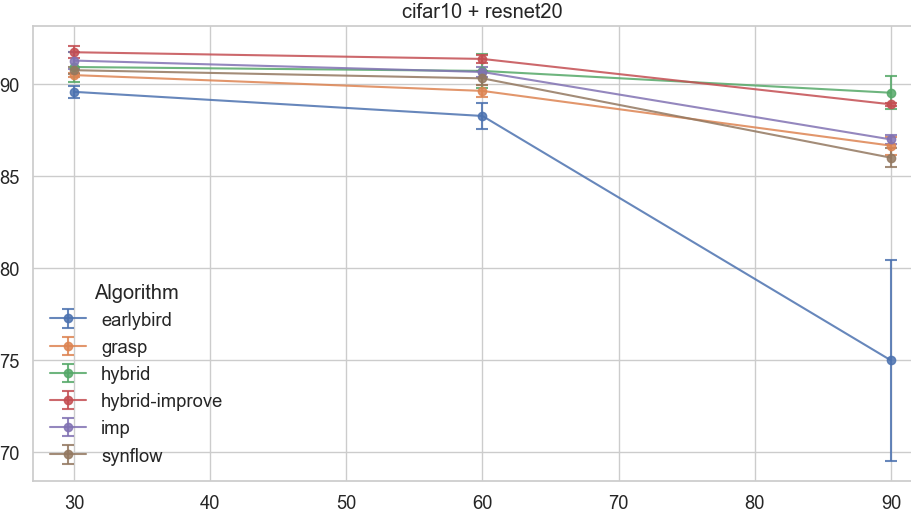
\includegraphics[width=0.9\textwidth]{image/resnet20-cifar10_acc+sparsity.png}
                \caption{Độ chính xác theo mức độ thưa trên CIFAR-10/ResNet-20}
                \label{fig:r20c10_heatmap_s03}
        \end{figure}
}

\frame{
    \frametitle{Thực nghiệm}
    \framesubtitle{Kết quả -- CIFAR-10 / ResNet-20: Độ chính xác theo độ thưa}
    \textbf{Hai nhóm hành vi quan sát được:}
    \vspace{0.2cm}
    \begin{block}{Nhóm suy giảm từ từ}
        GraSP, SynFlow, Hybrid, \textbf{Hybrid-Improve}, IMP: duy trì độ chính xác 85\%--91.5\% qua tất cả các mức $S$.
        \begin{itemize}
            \item Tại $S=0.30$: \textbf{Hybrid-Improve dẫn đầu} ($\approx$91.2\%), sụt giảm $\approx 0\%$
            \item Tại $S=0.90$: Hybrid và Hybrid-Improve dẫn đầu ($\approx$89\%--89.5\%)
        \end{itemize}
    \end{block}
    \begin{block}{Nhóm sụp đổ hiệu năng}
        \textbf{Early-Bird}: $\approx$89.5\% tại $S=0.30$ $\to$ $\approx$75\% tại $S=0.90$ (mất $>$16 điểm \%)
        \begin{itemize}
            \item Độ lệch chuẩn $\approx$5\%--6\% ở $S=0.90$ -- \textbf{không ổn định} giữa các seed
        \end{itemize}
    \end{block}
}

\frame{
    \frametitle{Thực nghiệm}
    \framesubtitle{Kết quả -- CIFAR-10 / ResNet-20: Độ chính xác theo độ thưa}
        \begin{figure}[h]
            \centering
                \centering
                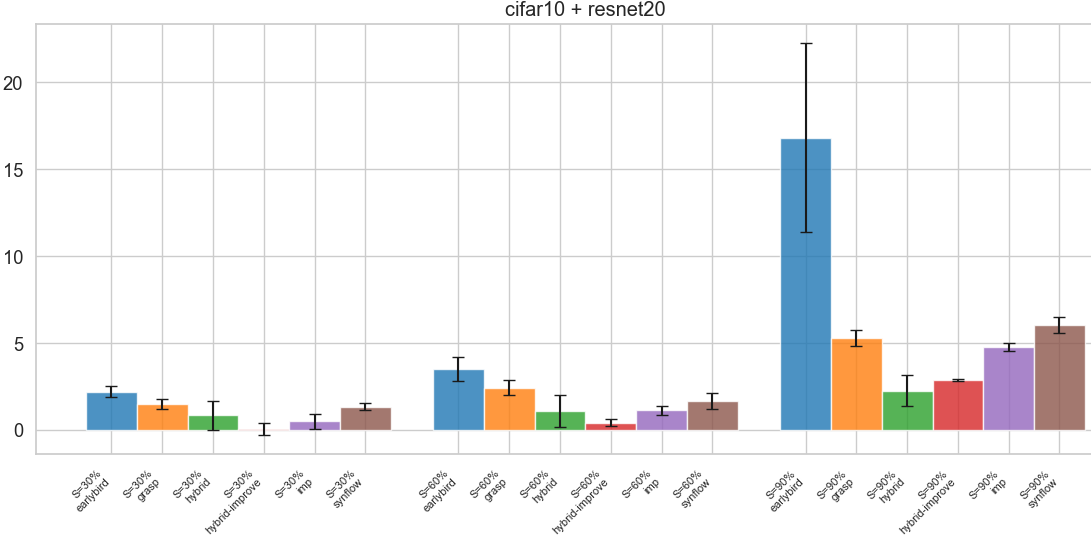
\includegraphics[width=\textwidth]{image/resnet20-cifar10_accdrop.png}
                \caption{Mức giảm độ chính xác so với mô hình dày đặc trên CIFAR-10/ResNet-20}
                \label{fig:r20c10_heatmap_s03}
        \end{figure}
}
\frame{
    \frametitle{Thực nghiệm}
    \framesubtitle{Kết quả -- CIFAR-10 / ResNet-20: Mức giảm độ chính xác}
    \begin{center}
    \begin{tabular}{lcccc}
        \toprule
        \textbf{Thuật toán} & $S=0.30$ & $S=0.60$ & $S=0.90$ & $\sigma$ tại 0.90 \\
        \midrule
        Hybrid-Improve & $\approx$0.0\% & $\approx$0.5\% & $\approx$3.0\% & \textbf{thấp} \\
        Hybrid         & $\approx$0.9\% & $\approx$1.1\% & $\approx$2.2\% & trung bình \\
        IMP            & $\approx$0.5\% & $\approx$1.3\% & $\approx$5.0\% & thấp \\
        GraSP          & $\approx$1.5\% & $\approx$2.4\% & $\approx$5.5\% & thấp \\
        SynFlow        & $\approx$1.4\% & $\approx$1.7\% & $\approx$6.2\% & cao \\
        Early-Bird     & $\approx$2.0\% & $\approx$3.5\% & $\approx$17\% & \textbf{rất cao} \\
        \bottomrule
    \end{tabular}
    \end{center}
    \vspace{0.3cm}
    \begin{itemize}
        \item \textbf{Hybrid} dẫn về trung bình tại $S=0.90$, nhưng \textbf{Hybrid-Improve ổn định hơn} (biên độ nhỏ hơn đáng kể)
        \item $S=0.30$: tất cả các phương pháp cắt tỉa không có cấu trúc đều trong vùng nén an toàn
    \end{itemize}
}

% =========================================================
% CIFAR-10 / ResNet-20 -- Pareto
% =========================================================

\frame{
    \frametitle{Thực nghiệm}
    \framesubtitle{CIFAR-10 / ResNet-20: Biên Pareto}

    \begin{figure}
        \centering
        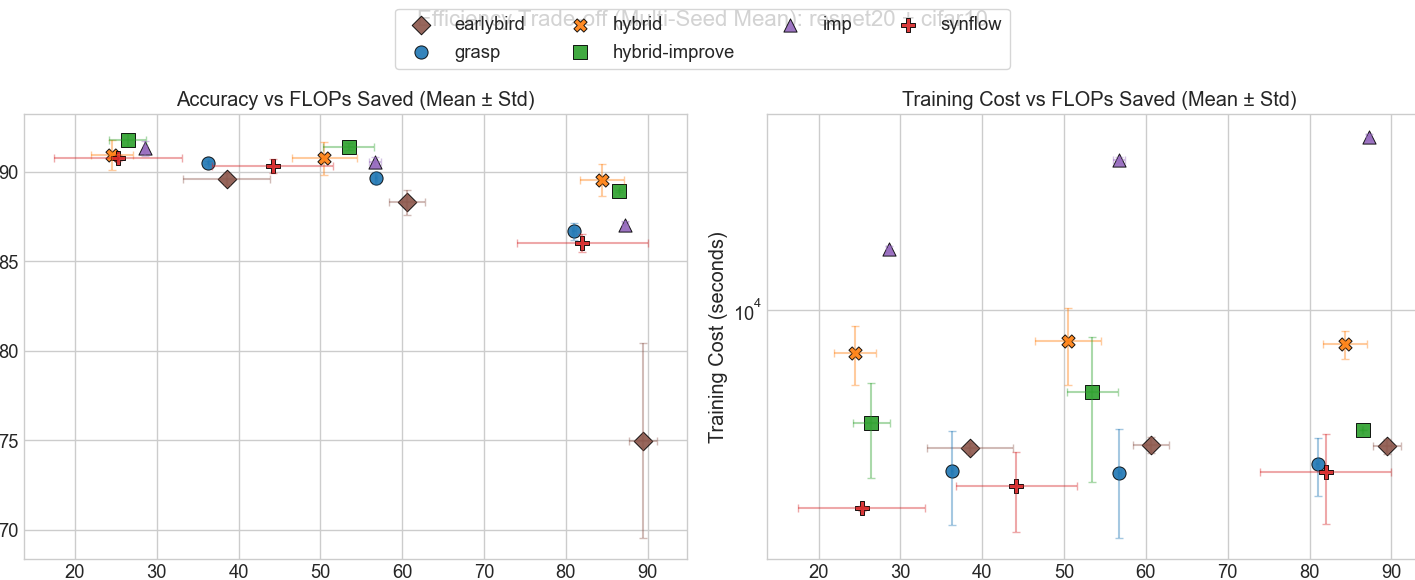
\includegraphics[width=0.92\textwidth]{image/resnet20-cifar10_pareto.png}
        \caption{Biểu đồ Pareto: Cân bằng giữa độ chính xác, FLOPs và chi phí huấn luyện trên CIFAR-10/ResNet-20}
        \label{fig:r20c10_pareto}
    \end{figure}
}

\frame{
    \frametitle{Thực nghiệm}
    \framesubtitle{CIFAR-10 / ResNet-20: Phân tích Pareto}

    \begin{itemize}
        \item Ở mức nén nhẹ, \textbf{Hybrid-Improve} đạt độ chính xác cao nhất và gần như không mất accuracy.
        \item Khi FLOPs saved $>80\%$, \textbf{Hybrid} và \textbf{Hybrid-Improve} nằm trên biên Pareto với $\approx 89\%$--$89.5\%$ accuracy.
        \item \textbf{GraSP} và \textbf{SynFlow} có chi phí huấn luyện thấp hơn, nhưng accuracy thấp hơn ở độ thưa cao.
        \item \textbf{IMP} có chi phí huấn luyện lớn nhất do nhiều vòng prune--retrain--rewind.
    \end{itemize}
}

% =========================================================
% CIFAR-10 / ResNet-20 -- Sparsity distribution
% =========================================================

\frame{
    \frametitle{Thực nghiệm}
    \framesubtitle{CIFAR-10 / ResNet-20: Phân phối độ thưa theo tầng}
    \begin{figure}
        \centering
        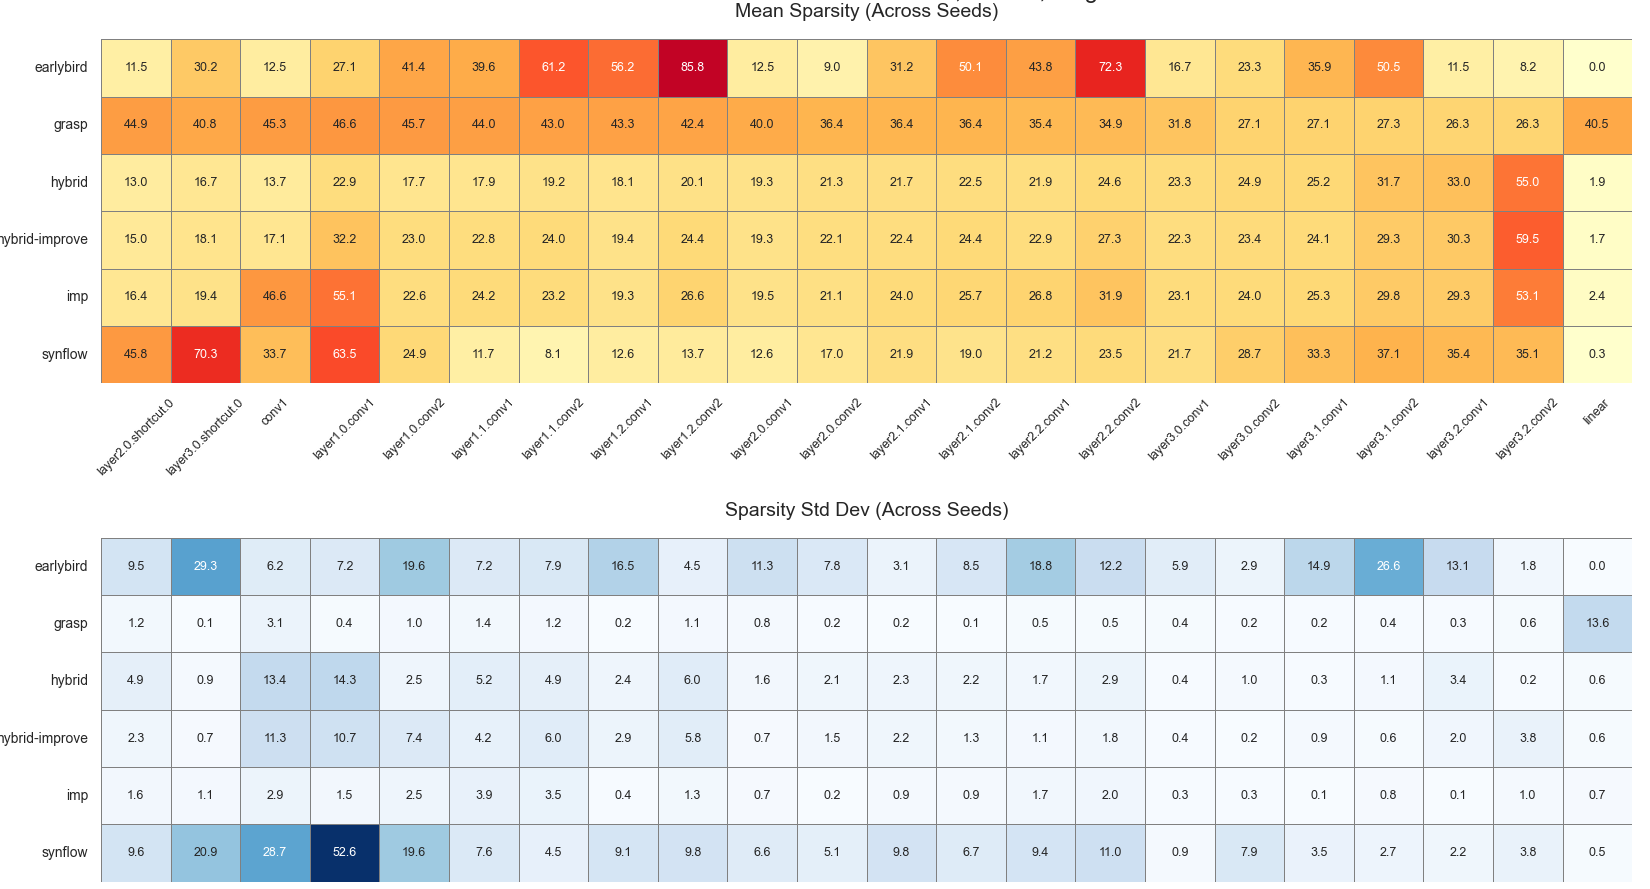
\includegraphics[width=0.9\textwidth]{image/resnet20-cifar10_s0.3_heatmap.png}
        \caption{ Bản đồ nhiệt phân phối độ thưa theo tầng trên CIFAR-10/ResNet-20 $S=0{,}30$}
    \end{figure}
}

\frame{
    \frametitle{Thực nghiệm}
    \framesubtitle{CIFAR-10 / ResNet-20: Phân phối độ thưa theo tầng}
    \begin{figure}
        \centering
        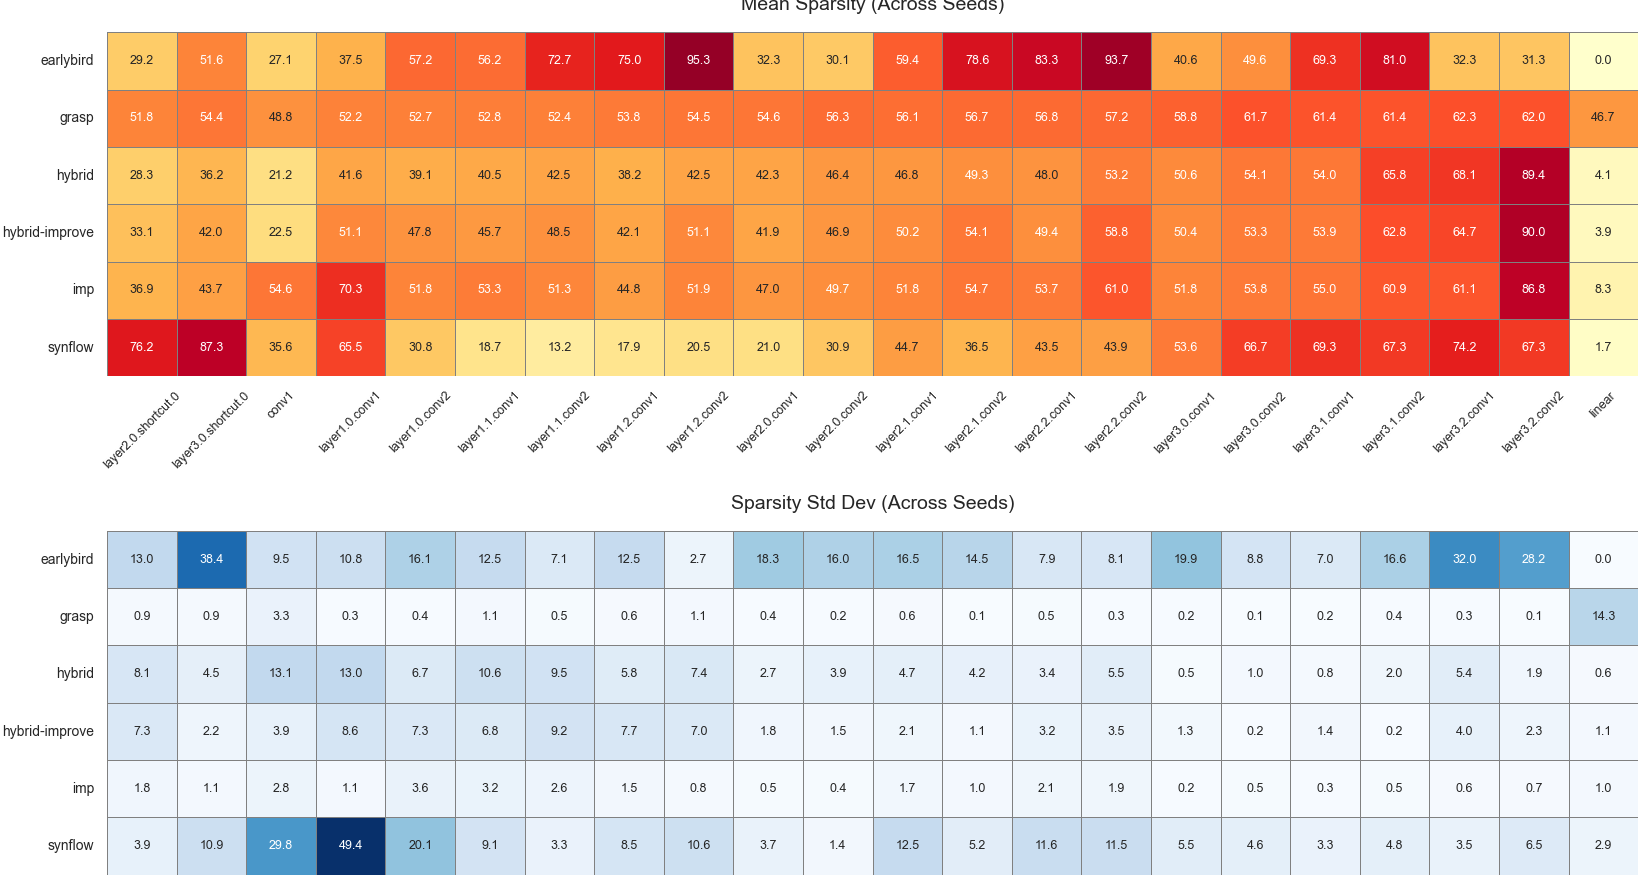
\includegraphics[width=0.9\textwidth]{image/resnet20-cifar10_s0.6_heatmap.png}
        \caption{ Bản đồ nhiệt phân phối độ thưa theo tầng trên CIFAR-10/ResNet-20 $S=0{,}60$}
    \end{figure}
}

\frame{
    \frametitle{Thực nghiệm}
    \framesubtitle{CIFAR-10 / ResNet-20: Phân phối độ thưa theo tầng}
    \begin{figure}
        \centering
        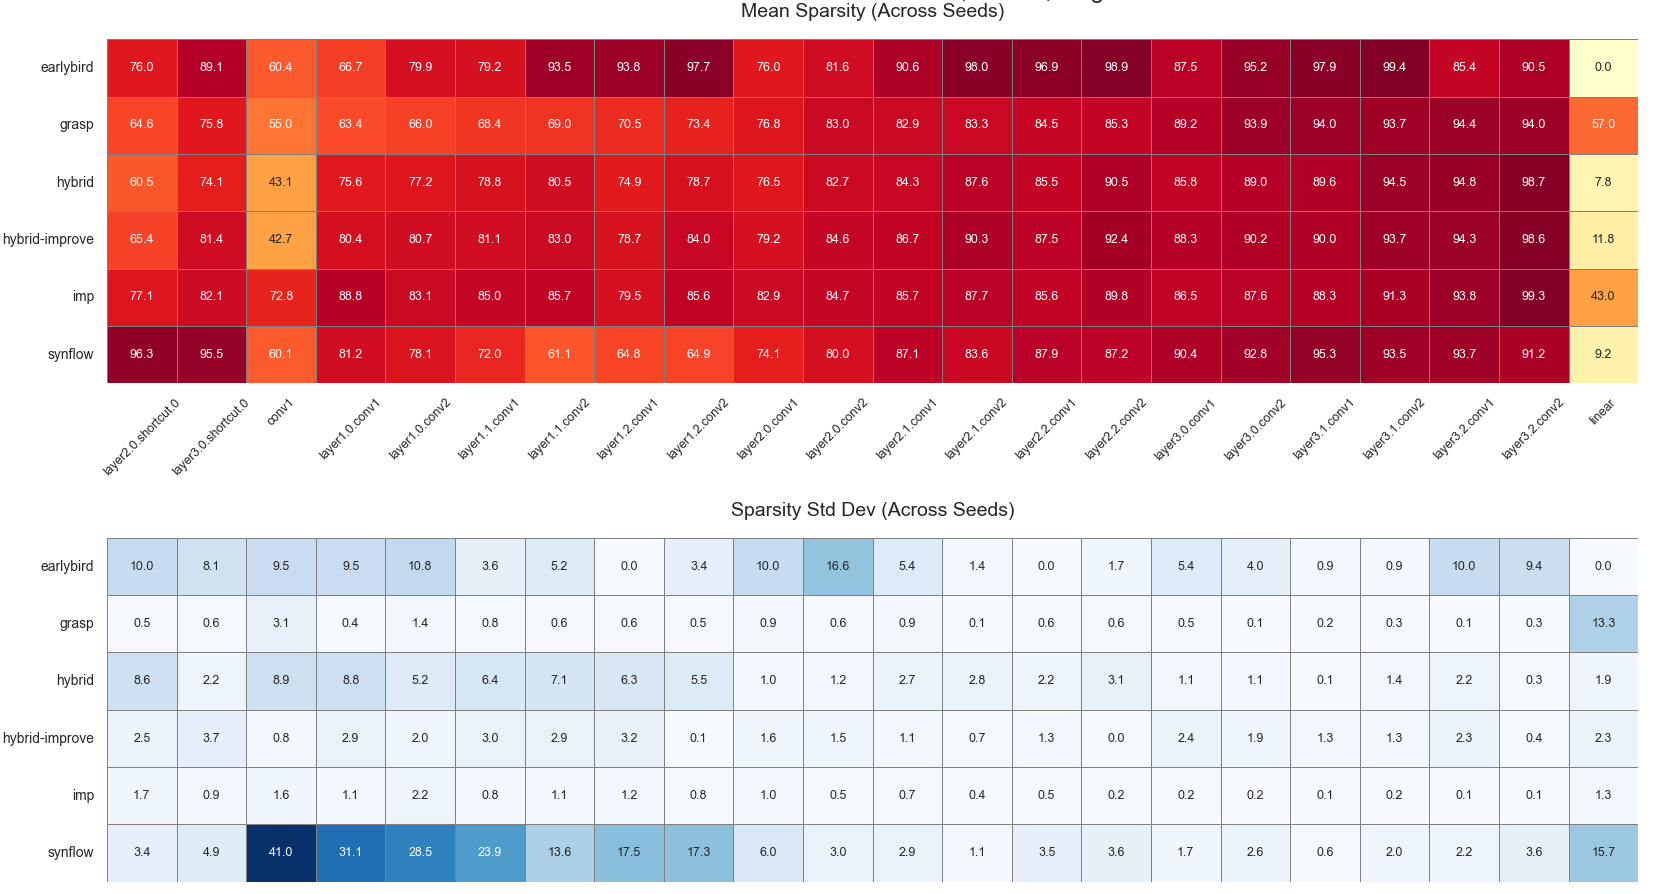
\includegraphics[width=0.9\textwidth]{image/resnet20-cifar10_s0.9_heatmap.png}
        \caption{ Bản đồ nhiệt phân phối độ thưa theo tầng trên CIFAR-10/ResNet-20 $S=0{,}90$}
    \end{figure}
}

\frame{
    \frametitle{Thực nghiệm}
    \framesubtitle{CIFAR-10 / ResNet-20: Nhận xét phân phối độ thưa}

    \begin{columns}
        \column{0.5\textwidth}
        \textbf{Ổn định hơn}
        \begin{itemize}
            \item \textbf{GraSP}: phân phối đều nhất qua các tầng.
            \item \textbf{Hybrid-Improve}: bảo vệ tầng đầu tốt hơn, tránh cắt tỉa quá mạnh ở vùng nhạy cảm.
            \item \textbf{Hybrid}: phân phối tương tự Hybrid-Improve nhưng kém ổn định hơn.
        \end{itemize}

        \column{0.5\textwidth}
        \textbf{Dễ mất ổn định}
        \begin{itemize}
            \item \textbf{SynFlow}: biến động lớn giữa các seed ở một số tầng đầu.
            \item \textbf{Early-Bird}: BN $\gamma$ chưa đủ tin cậy ở độ thưa cao.
            \item Ở $S=0{,}90$, phân phối lệch mạnh dễ kéo theo sụt giảm accuracy.
        \end{itemize}
    \end{columns}
}

\frame{
    \frametitle{Thực nghiệm}
    \framesubtitle{Kết quả -- CIFAR-100 / ResNet-20}
            \begin{figure}[h]
            \centering
            \begin{subfigure}{0.49\textwidth}
                \centering
                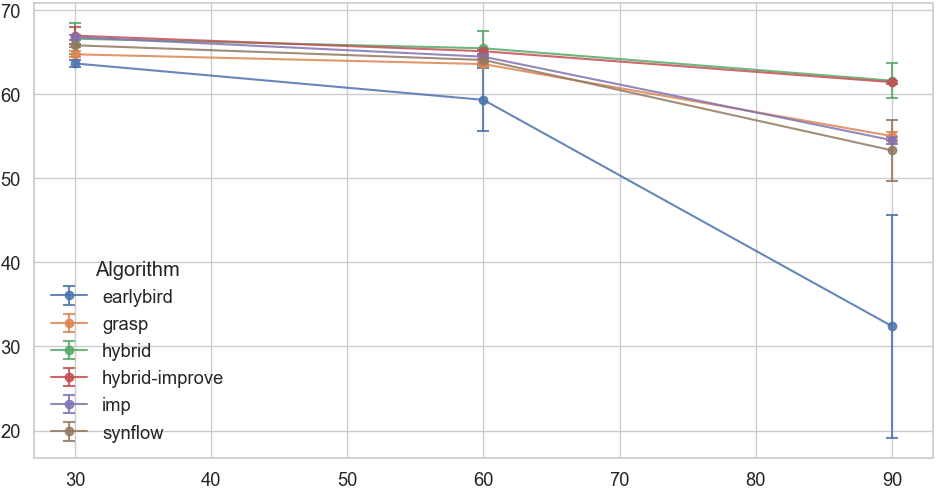
\includegraphics[width=\textwidth]{image/resnet20-cifar100_acc+sparsity.png}
                \caption{Độ chính xác theo mức độ thưa trên CIFAR-100/ResNet-20}
                \label{fig:r20c10_heatmap_s03}
            \end{subfigure}
            \hfill
            \begin{subfigure}{0.49\textwidth}
                \centering
                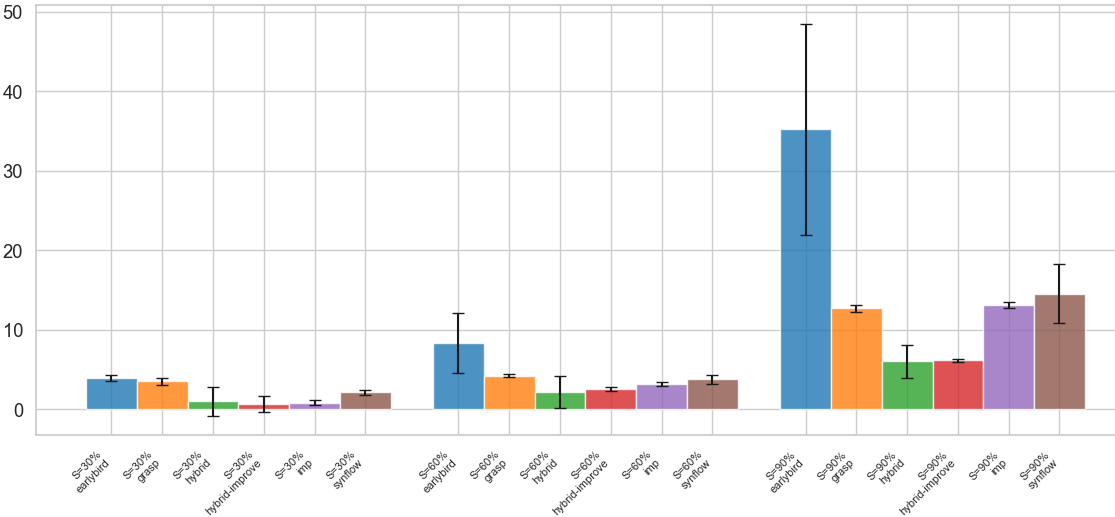
\includegraphics[width=\textwidth]{image/resnet20-cifar100_accdrop.png}
                \caption{Mức giảm độ chính xác so với mô hình dày đặc trên CIFAR-100/ResNet-20}
                \label{fig:r20c10_heatmap_s06}
            \end{subfigure}
            \label{fig:grouped-accuracy}
        \end{figure}
}

\frame{
    \frametitle{Thực nghiệm}
    \framesubtitle{Kết quả -- CIFAR-100 / ResNet-20}
    \textbf{CIFAR-100 khó hơn đáng kể:} 100 lớp, ít dữ liệu/lớp hơn $\Rightarrow$ mức sụt giảm lớn hơn.
    \vspace{0.3cm}
    \begin{itemize}
        \item Tại $S=0.30$: Hybrid-Improve ($\approx$0.7\%) và Hybrid ($\approx$1.0\%) vẫn giữ hiệu suất tốt nhất
        \item Tại $S=0.60$: Early-Bird sụt giảm $\approx$8.5\% với thanh lỗi lớn
        \item Tại $S=0.90$:
        \begin{itemize}
            \item \textbf{Early-Bird sụp đổ}: $\approx$35\% sụt giảm, $\sigma \approx 13\%$ $\Rightarrow$ độ chính xác có thể $< 20\%$
            \item GraSP và IMP: $\approx$13\%, SynFlow: $\approx$14.5\%
            \item \textbf{Hybrid và Hybrid-Improve dẫn đầu}: $\approx$6\% sụt giảm
        \end{itemize}
    \end{itemize}
    \vspace{0.2cm}
}

% =========================================================
% CIFAR-100 / ResNet-20 -- Pareto
% =========================================================

\frame{
    \frametitle{Thực nghiệm}
    \framesubtitle{CIFAR-100 / ResNet-20: Biên Pareto}

    \begin{figure}
        \centering
        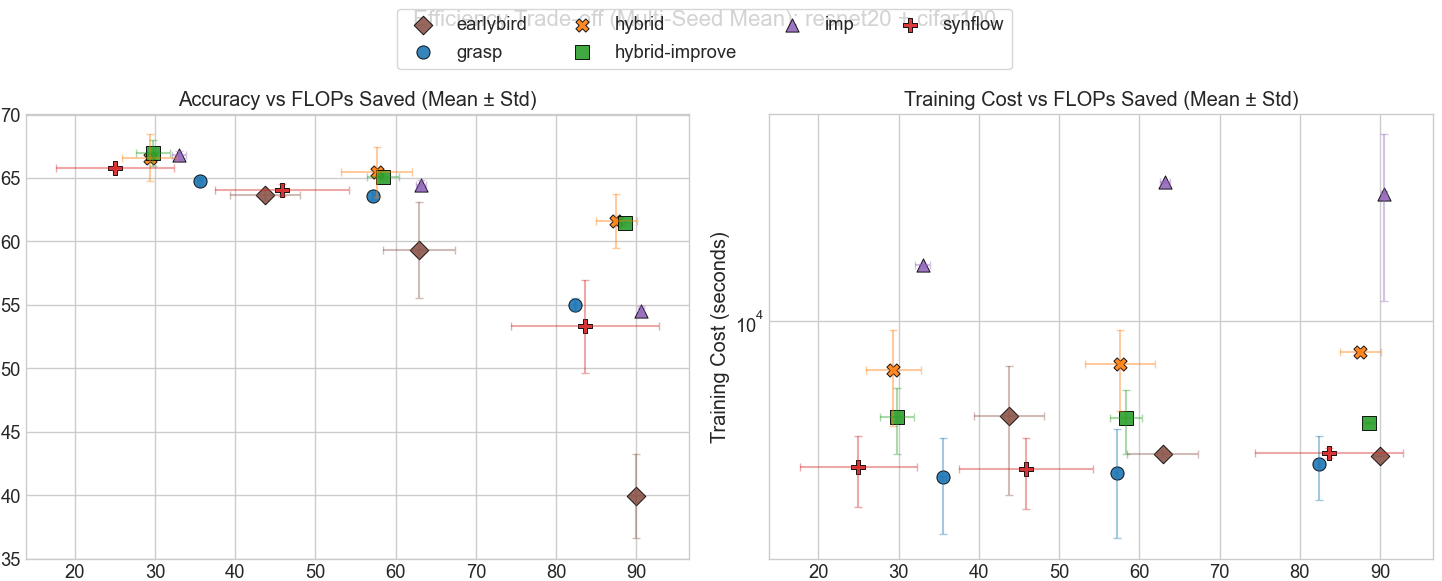
\includegraphics[width=0.92\textwidth]{image/resnet20-cifar100_pareto.png}
        \caption{Biểu đồ Pareto: Cân bằng giữa độ chính xác, FLOPs và chi phí huấn luyện trên CIFAR-100/ResNet-20}
        \label{fig:r20c100_pareto}
    \end{figure}
}

\frame{
    \frametitle{Thực nghiệm}
    \framesubtitle{CIFAR-100 / ResNet-20: Phân tích Pareto}

    \begin{itemize}
        \item Dải accuracy thấp hơn CIFAR-10 do bài toán 100 lớp khó hơn.
        \item Tại FLOPs saved $>80\%$, \textbf{Hybrid} và \textbf{Hybrid-Improve} đạt khoảng $\approx 61.5\%$ accuracy.
        \item \textbf{GraSP} rẻ hơn nhưng accuracy thấp hơn rõ rệt ở độ thưa cao.
        \item \textbf{IMP} có chi phí cao nhưng không tạo lợi thế tương xứng ở $S=0{,}90$.
        \item \textbf{Early-Bird} không nằm trên biên Pareto do sụp đổ accuracy mạnh.
    \end{itemize}
}

% =========================================================
% CIFAR-100 / ResNet-20 -- Sparsity distribution
% =========================================================

\frame{
    \frametitle{Thực nghiệm}
    \framesubtitle{CIFAR-100 / ResNet-20: Phân phối độ thưa theo tầng}
    \begin{figure}
        \centering
        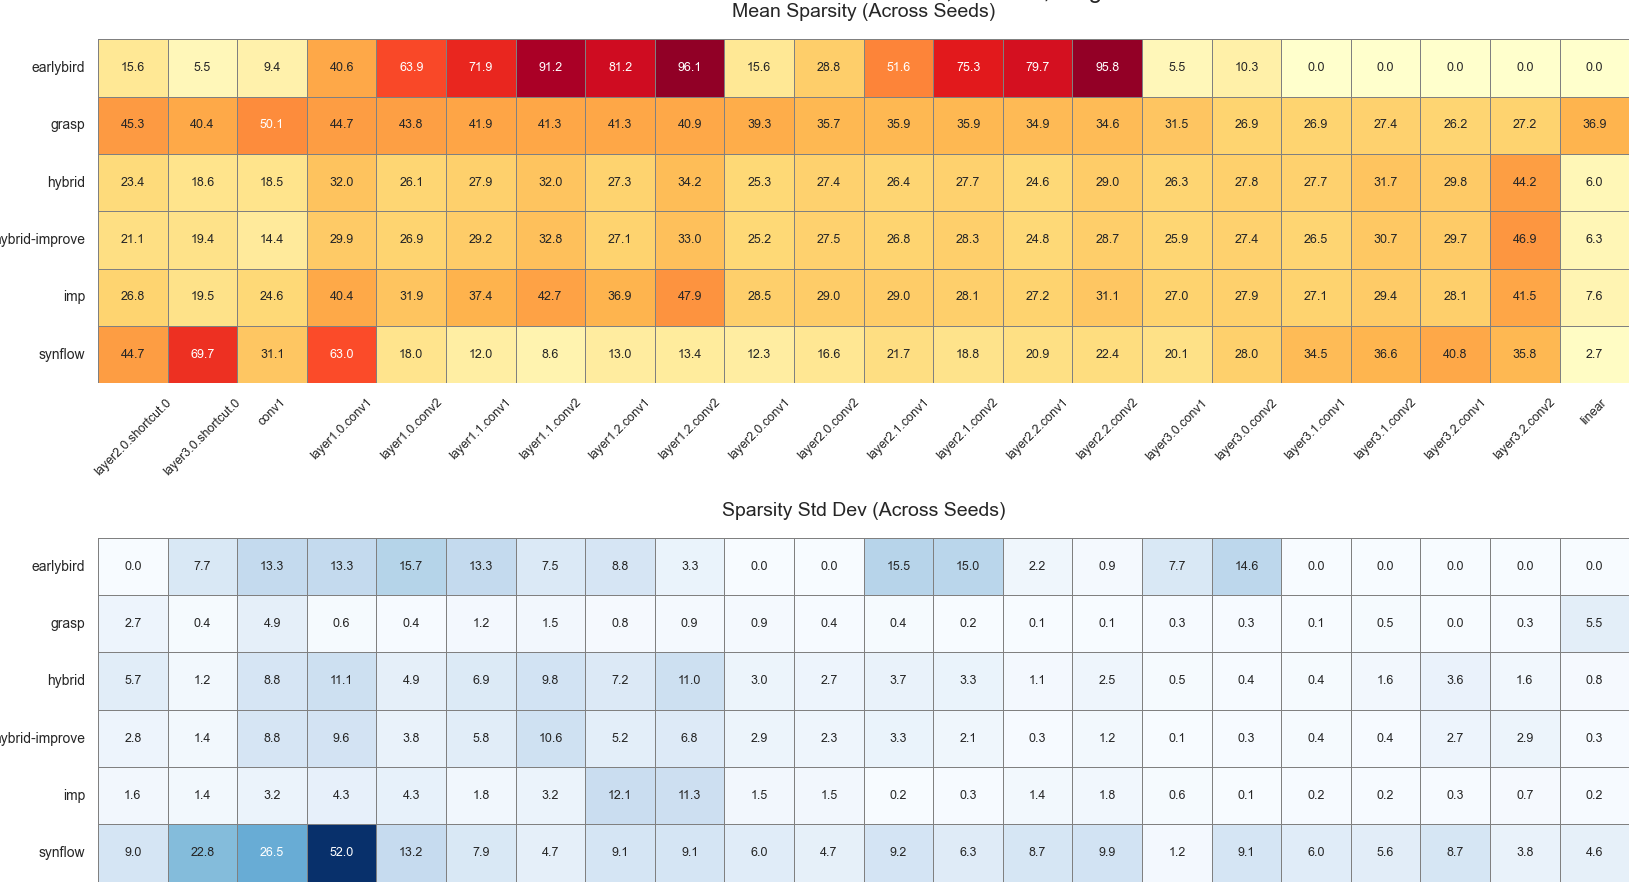
\includegraphics[width=0.9\textwidth]{image/resnet20-cifar100_s0.3_heatmap.png}
        \caption{ Bản đồ nhiệt phân phối độ thưa theo tầng trên CIFAR-100/ResNet-20 $S=0{,}30$}
    \end{figure}
}

\frame{
    \frametitle{Thực nghiệm}
    \framesubtitle{CIFAR-100 / ResNet-20: Phân phối độ thưa theo tầng}
    \begin{figure}
        \centering
        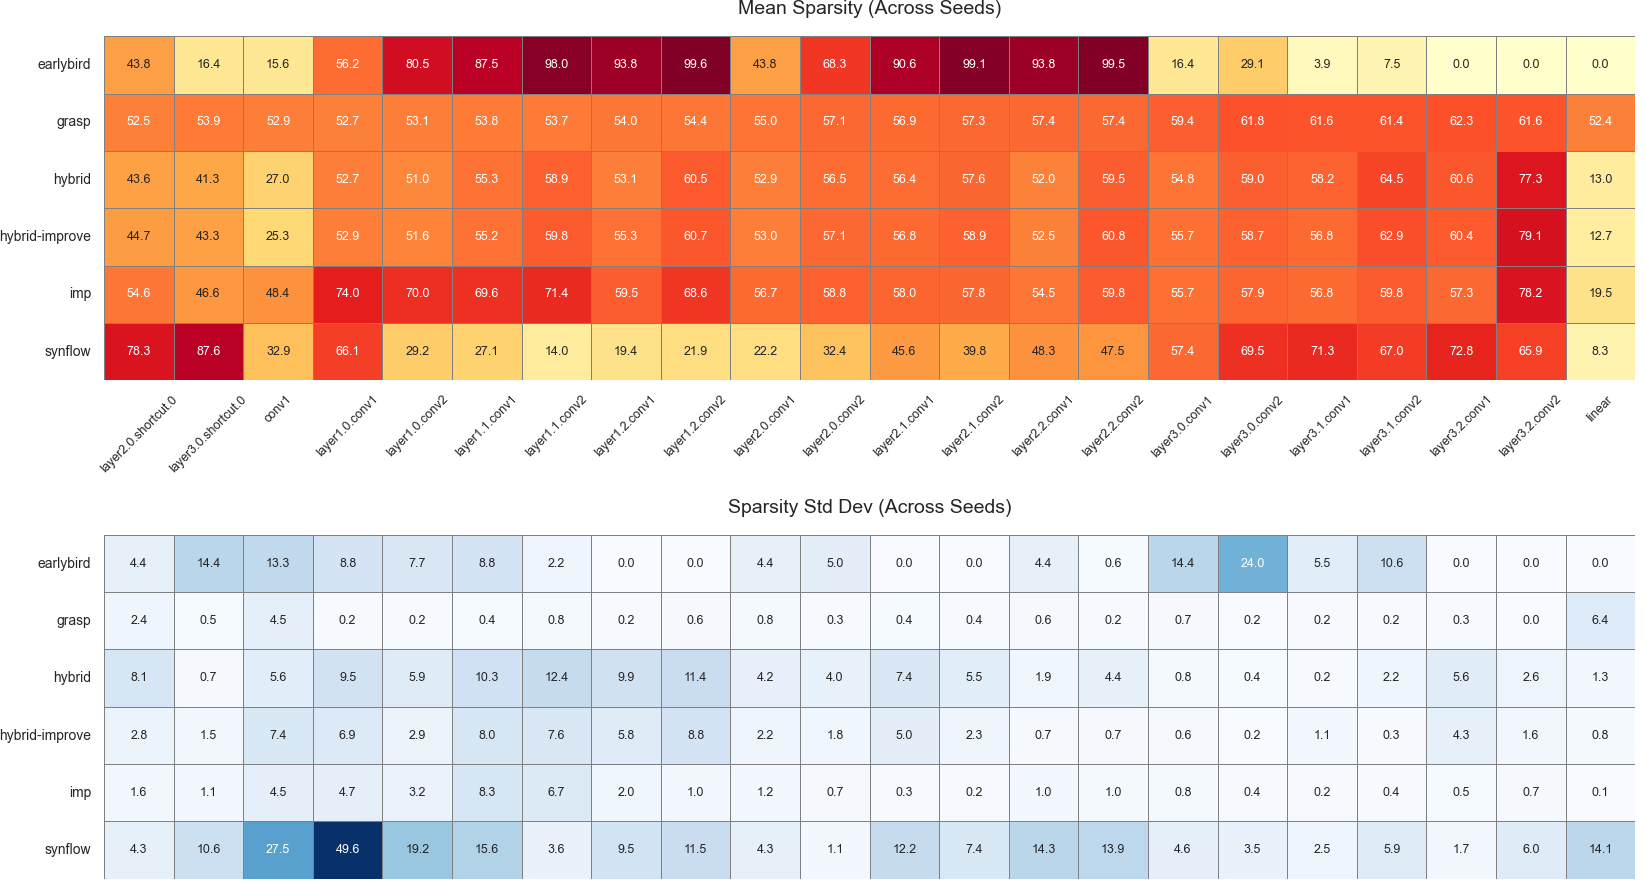
\includegraphics[width=0.9\textwidth]{image/resnet20-cifar100_s0.6_heatmap.png}
        \caption{ Bản đồ nhiệt phân phối độ thưa theo tầng trên CIFAR-100/ResNet-20 $S=0{,}60$}
    \end{figure}
}

\frame{
    \frametitle{Thực nghiệm}
    \framesubtitle{CIFAR-100 / ResNet-20: Phân phối độ thưa theo tầng}
    \begin{figure}
        \centering
        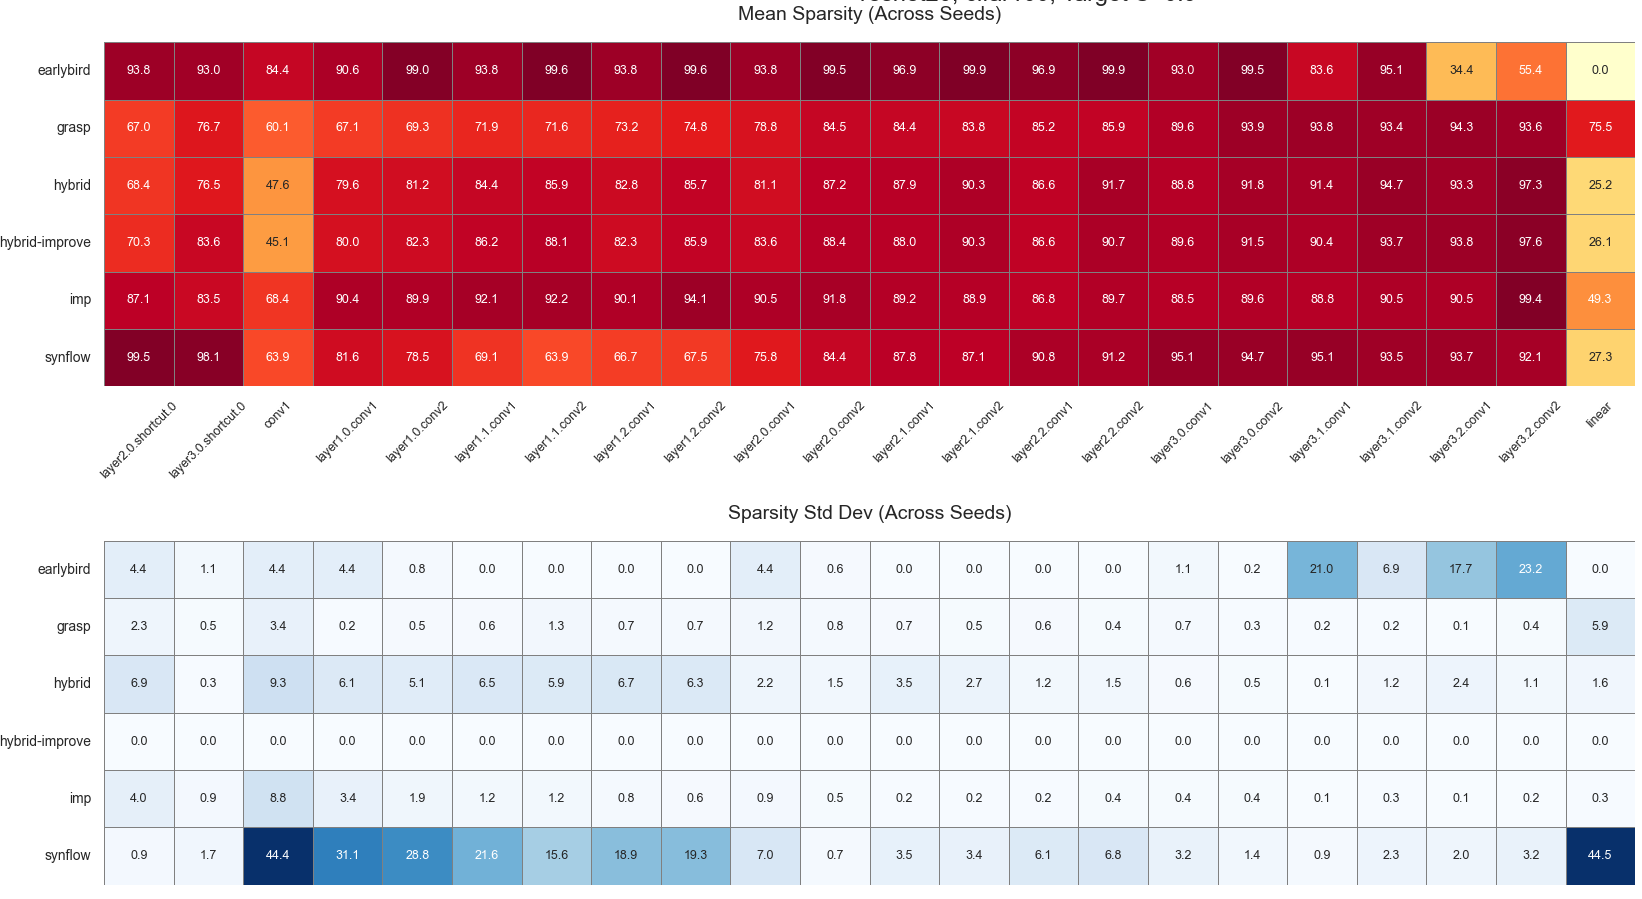
\includegraphics[width=0.9\textwidth]{image/resnet20-cifar100_s0.9_heatmap.png}
        \caption{ Bản đồ nhiệt phân phối độ thưa theo tầng trên CIFAR-100/ResNet-20 $S=0{,}90$}
    \end{figure}
}

\frame{
    \frametitle{Thực nghiệm}
    \framesubtitle{CIFAR-100 / ResNet-20: Nhận xét phân phối độ thưa}

    \begin{itemize}
        \item CIFAR-100 khó hơn CIFAR-10: ít dữ liệu/lớp hơn nên mạng ít dư thừa hơn.
        \item \textbf{Early-Bird} tạo phân phối thưa kênh nghiêm trọng hơn; nhiều tầng có độ thưa rất cao ngay cả ở mức nén nhẹ.
        \item \textbf{SynFlow} tiếp tục có độ lệch chuẩn cao ở các tầng đầu, cho thấy bất ổn do thuật toán chứ không chỉ do dữ liệu.
        \item \textbf{Hybrid} và \textbf{Hybrid-Improve} giữ phân phối cân bằng hơn, giúp duy trì accuracy tốt nhất ở $S=0{,}90$.
    \end{itemize}
}


\frame{
    \frametitle{Thực nghiệm}
    \framesubtitle{Kết quả -- CIFAR-10 / ResNet-50}
                \begin{figure}[h]
            \centering
            \begin{subfigure}{0.49\textwidth}
                \centering
                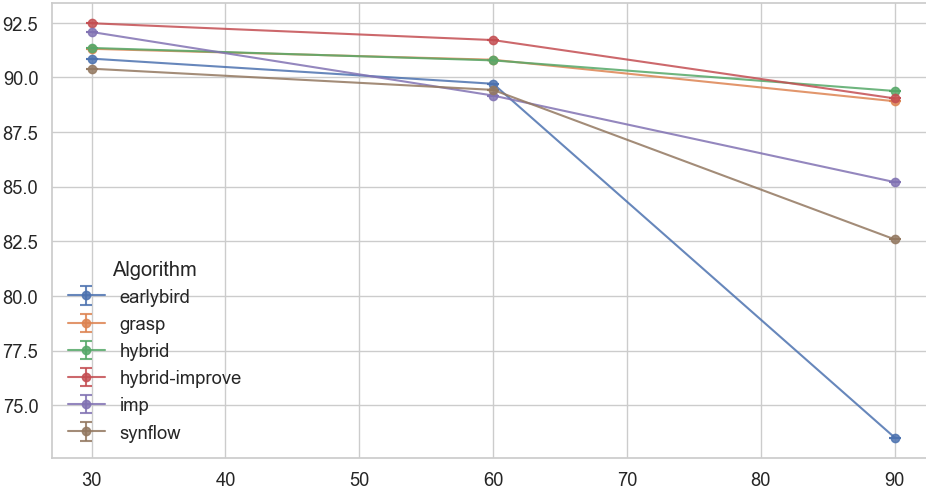
\includegraphics[width=\textwidth]{image/resnet50-cifar10_acc+sparsity.png}
                \caption{Độ chính xác theo mức độ thưa trên CIFAR-10/ResNet-50}
                \label{fig:r20c10_heatmap_s03}
            \end{subfigure}
            \hfill
            \begin{subfigure}{0.49\textwidth}
                \centering
                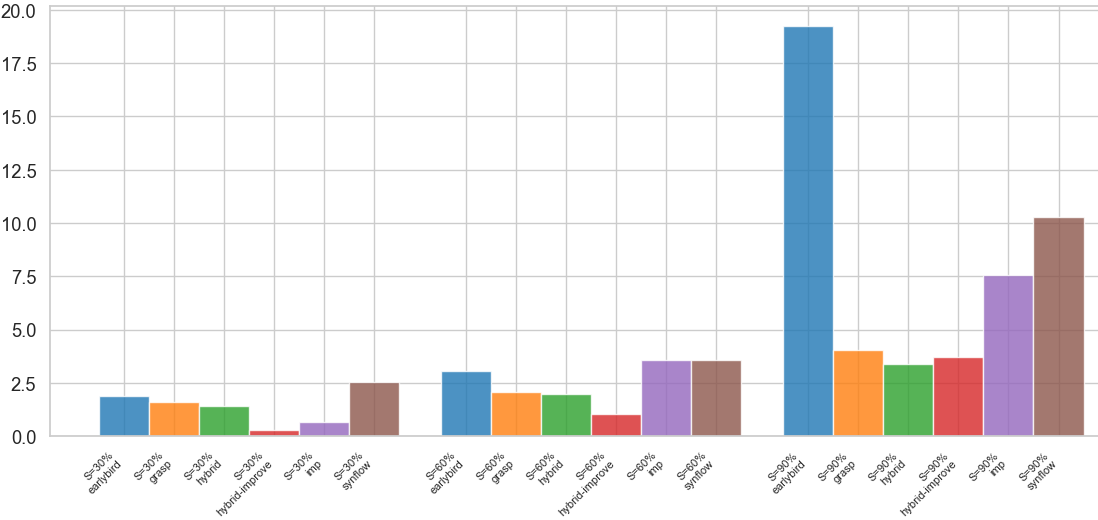
\includegraphics[width=\textwidth]{image/resnet50-cifar10_accdrop.png}
                \caption{Mức giảm độ chính xác so với mô hình dày đặc trên CIFAR-10/ResNet-50}
                \label{fig:r20c10_heatmap_s06}
            \end{subfigure}
            \label{fig:grouped-accuracy}
        \end{figure}
}

\frame{
    \frametitle{Thực nghiệm}
    \framesubtitle{Kết quả -- CIFAR-10 / ResNet-50}
    \begin{itemize}
        \item Tại $S=0.30$: Hybrid và Hybrid-Improve vẫn dẫn đầu với tỉ lệ giảm độ chính xác thấp nhất.
        \item Tại $S=0.90$: Hybrid ($\approx$3.3\%) và Hybrid-Improve ($\approx$3.5\%) -- \textbf{ổn định giữa các kiến trúc}
    \end{itemize}
    \vspace{0.2cm}
    \begin{alertblock}{Điểm đáng chú ý với ResNet-50}
        Trên ResNet-50, khoảng cách accuracy giữa \textbf{GraSP} và hybrid thu hẹp xuống $< 1\%$ tại $S=0.90$, trong khi chi phí huấn luyện vẫn chênh lớn. GraSP chiếm vị trí tốt hơn trên \textbf{biên Pareto} (accuracy vs. chi phí) ở kiến trúc sâu này.
    \end{alertblock}
    \vspace{0.1cm}
    \begin{itemize}
        \item SynFlow sụp đổ shortcut tại $S=0.90$: nhiều tầng shortcut đạt $\approx 99\%$--$100\%$ độ thưa
    \end{itemize}
}

% =========================================================
% CIFAR-10 / ResNet-50 -- Pareto
% =========================================================

\frame{
    \frametitle{Thực nghiệm}
    \framesubtitle{CIFAR-10 / ResNet-50: Biên Pareto}

    \begin{figure}
        \centering
        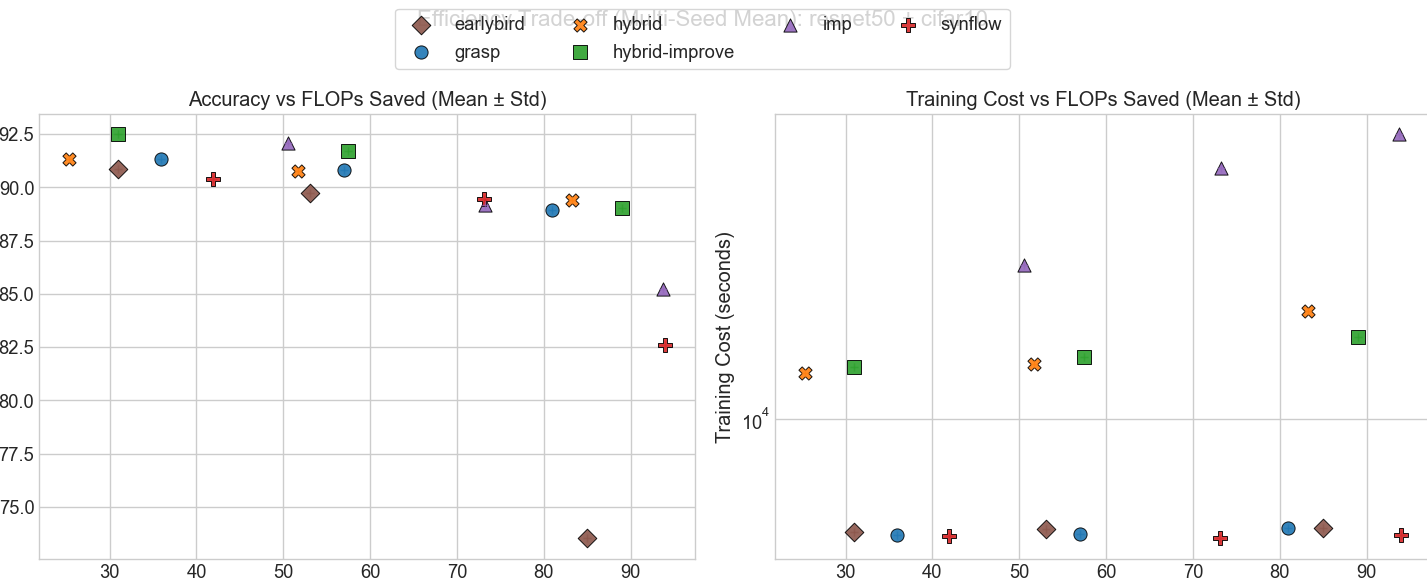
\includegraphics[width=0.92\textwidth]{image/resnet50-cifar10_pareto.png}
        \caption{Biểu đồ Pareto: Cân bằng giữa độ chính xác, FLOPs và chi phí huấn luyện trên CIFAR-10/ResNet-50}
        \label{fig:r50c10_pareto}
    \end{figure}
}

\frame{
    \frametitle{Thực nghiệm}
    \framesubtitle{CIFAR-10 / ResNet-50: Phân tích Pareto}

    \begin{itemize}
        \item \textbf{Hybrid} và \textbf{Hybrid-Improve} vẫn giữ accuracy cao tại $S=0{,}90$.
        \item Khoảng cách giữa \textbf{GraSP} và nhóm Hybrid thu hẹp trên ResNet-50.
        \item Do chi phí huấn luyện thấp hơn nhiều, \textbf{GraSP} trở thành lựa chọn cạnh tranh hơn trên biên Pareto.
        \item \textbf{SynFlow} bị hạn chế bởi xu hướng làm thưa quá mạnh các shortcut.
        \item \textbf{Early-Bird} tiếp tục kém phù hợp ở độ thưa cao do BN $\gamma$ ở giai đoạn sớm chưa ổn định.
    \end{itemize}
}

% =========================================================
% CIFAR-10 / ResNet-50 -- Sparsity distribution
% =========================================================

\frame{
    \frametitle{Thực nghiệm}
    \framesubtitle{CIFAR-10 / ResNet-50: Phân phối độ thưa theo tầng}

    \begin{figure}
            \centering
            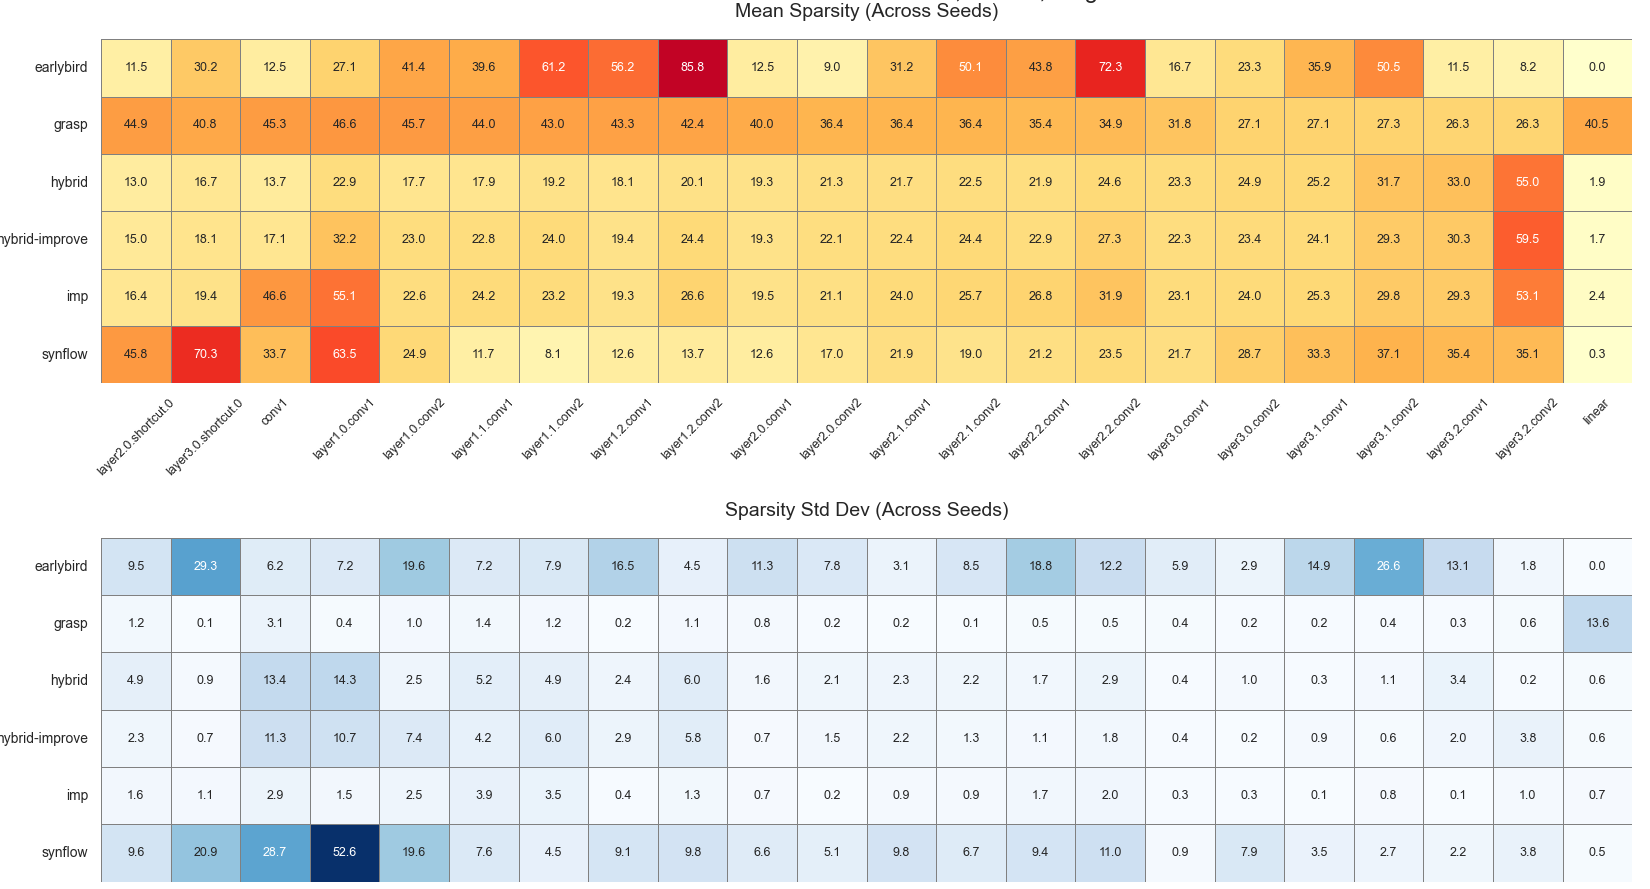
\includegraphics[width=0.9\textwidth]{image/resnet20-cifar10_s0.3_heatmap.png}
            \caption{Bản đồ nhiệt phân phối độ thưa theo tầng trên CIFAR-10/ResNet-50 $S=0{,}30$}
            \label{fig:r50c10_sparsity_dist_s03}
    \end{figure}
}
\frame{
    \frametitle{Thực nghiệm}
    \framesubtitle{CIFAR-10 / ResNet-50: Phân phối độ thưa theo tầng}

    \begin{figure}
            \centering
            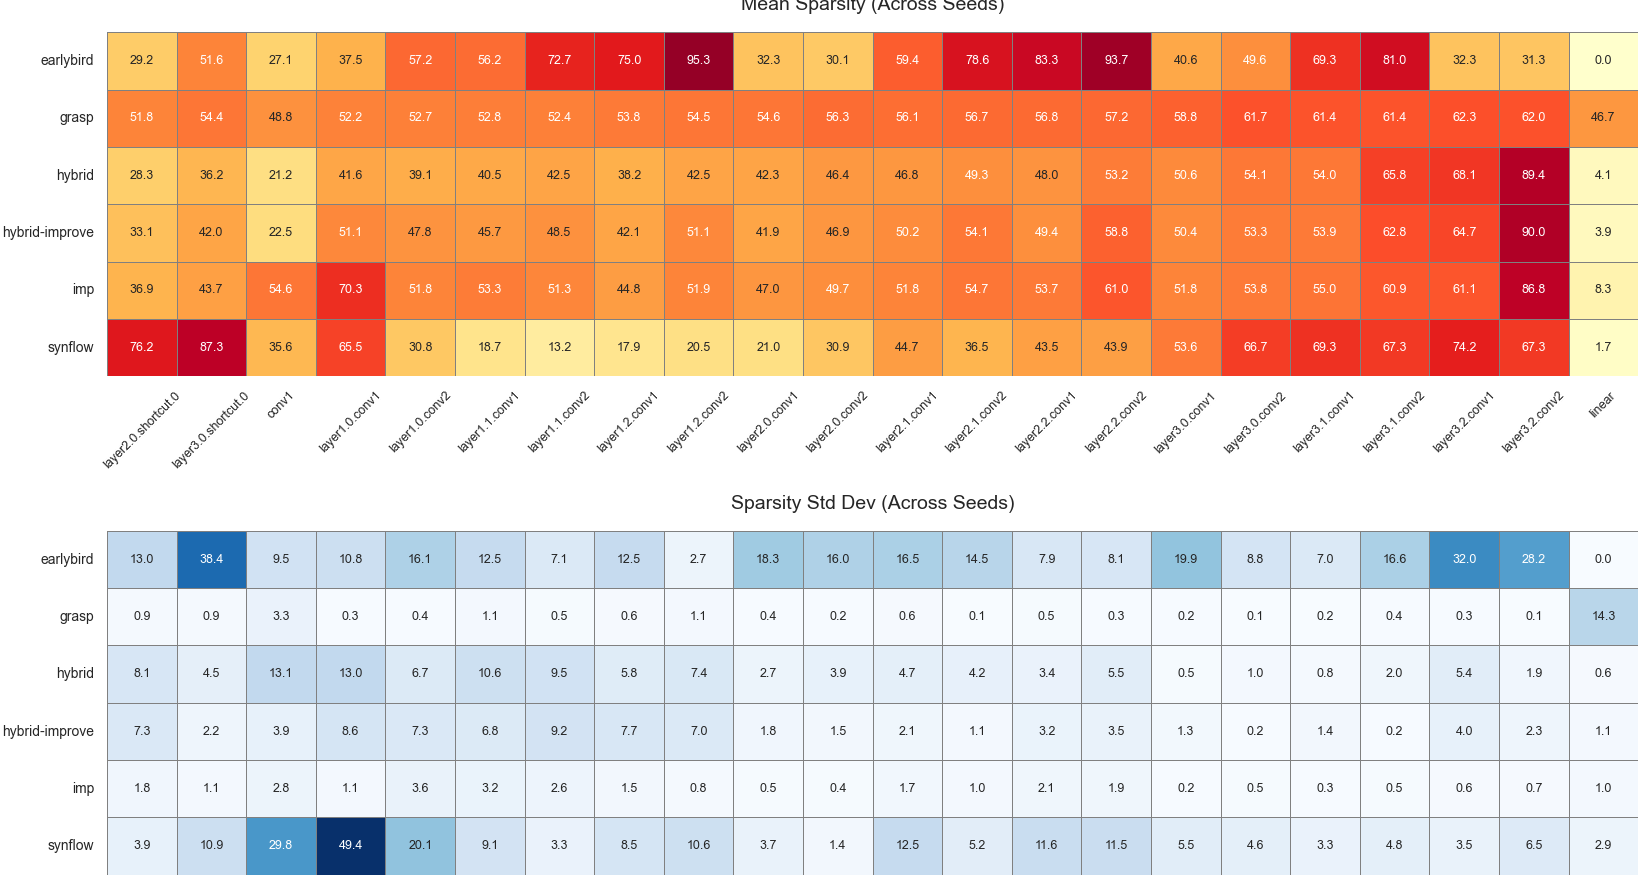
\includegraphics[width=0.9\textwidth]{image/resnet20-cifar10_s0.6_heatmap.png}
            \caption{Bản đồ nhiệt phân phối độ thưa theo tầng trên CIFAR-10/ResNet-50 $S=0{,}60$}
            \label{fig:r50c10_sparsity_dist_s03}
    \end{figure}
}
\frame{
    \frametitle{Thực nghiệm}
    \framesubtitle{CIFAR-10 / ResNet-50: Phân phối độ thưa theo tầng}

    \begin{figure}
            \centering
            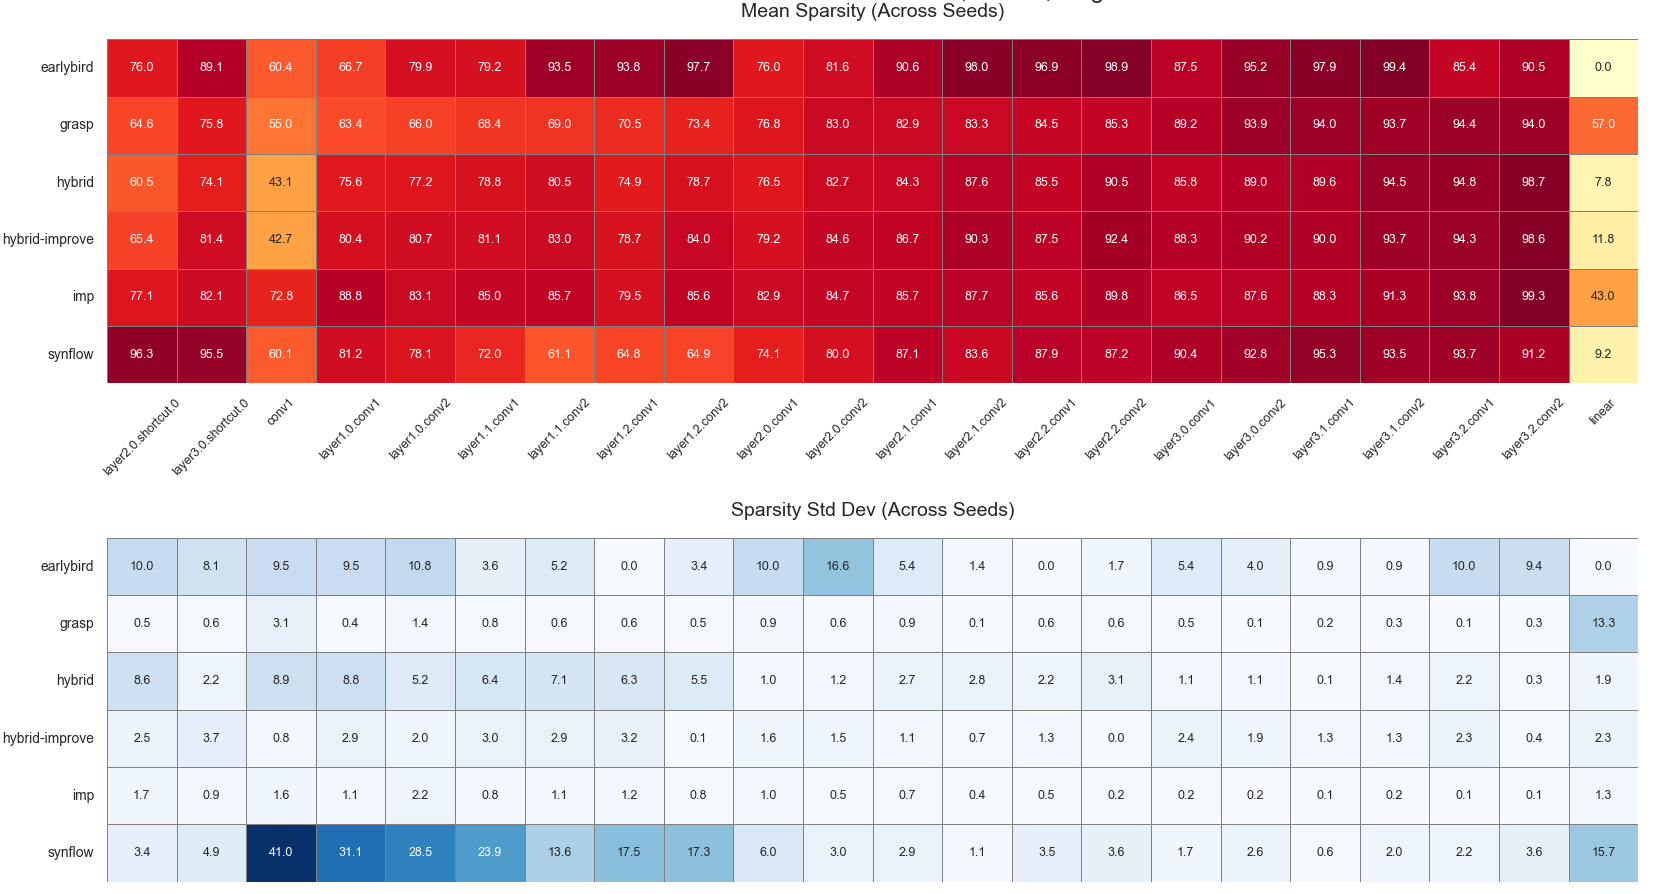
\includegraphics[width=0.9\textwidth]{image/resnet20-cifar10_s0.9_heatmap.png}
            \caption{Bản đồ nhiệt phân phối độ thưa theo tầng trên CIFAR-10/ResNet-50 $S=0{,}90$}
            \label{fig:r50c10_sparsity_dist_s03}
    \end{figure}
}

\frame{
    \frametitle{Thực nghiệm}
    \framesubtitle{CIFAR-10 / ResNet-50: Nhận xét phân phối độ thưa}

    \begin{itemize}
        \item Các mô hình phân phối tương tự ResNet-20 nhưng cường độ mạnh hơn do kiến trúc sâu hơn.
        \item \textbf{SynFlow} tập trung độ thưa vào các shortcut $1\times1$; tại $S=0{,}90$, nhiều shortcut gần $100\%$ độ thưa.
        \item \textbf{IMP} cũng đẩy một số tầng shortcut đầu lên độ thưa rất cao ngay cả tại $S=0{,}30$.
        \item \textbf{GraSP} vẫn phân phối đều nhất, ít bị ảnh hưởng bởi kích thước tầng.
        \item \textbf{Hybrid} và \textbf{Hybrid-Improve} ổn định hơn giữa ResNet-20 và ResNet-50.
    \end{itemize}
}

\frame{
    \frametitle{Thực nghiệm}
    \framesubtitle{Độ trễ suy diễn và chi phí huấn luyện}
    \begin{figure}[h]
        \centering
        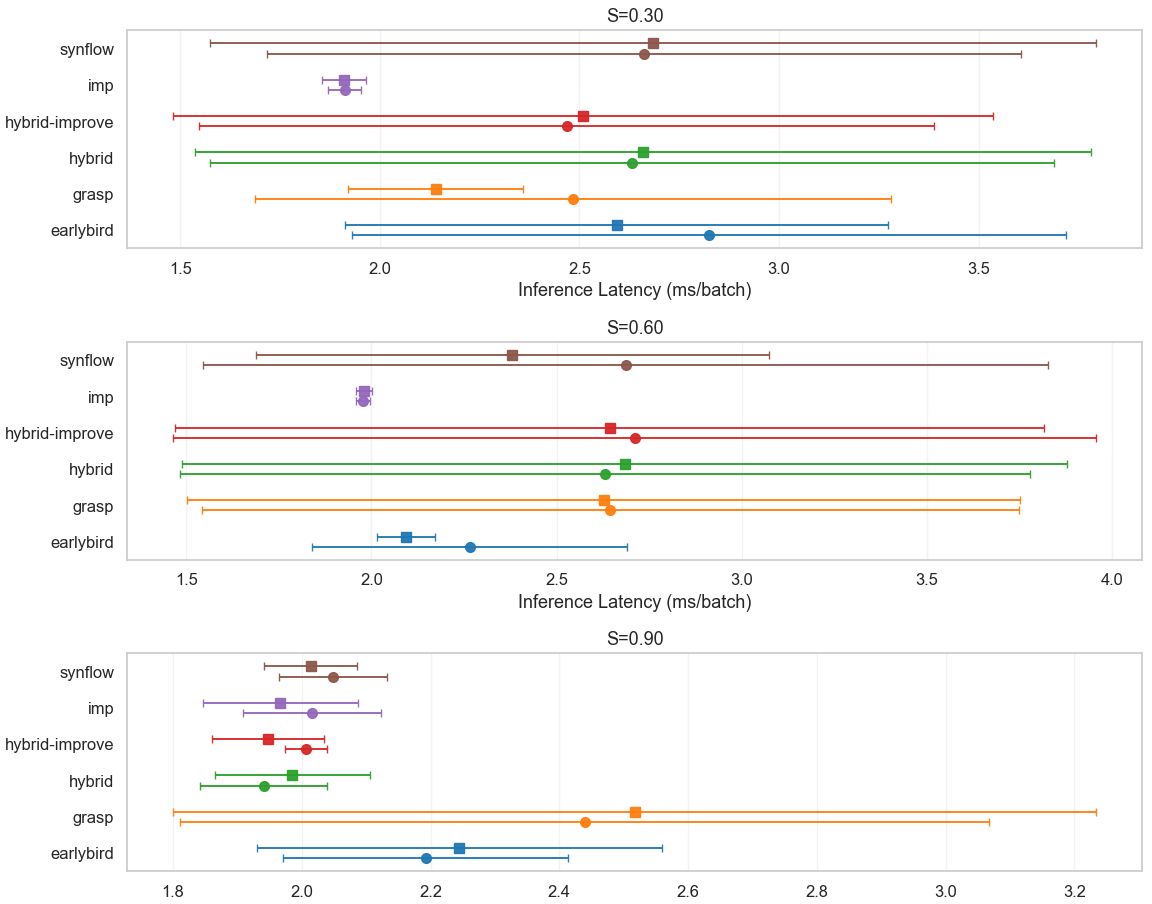
\includegraphics[width=0.7\textwidth]{image/resnet20-cifar10_latency.png}
        \caption{Độ trễ suy diễn theo mức độ thưa trên CIFAR-10/ResNet-20}
        \label{fig:r20c10_latency}
    \end{figure}
}

\frame{
    \frametitle{Thực nghiệm}
    \framesubtitle{Độ trễ suy diễn và chi phí huấn luyện}
    \begin{figure}[h]
        \centering
        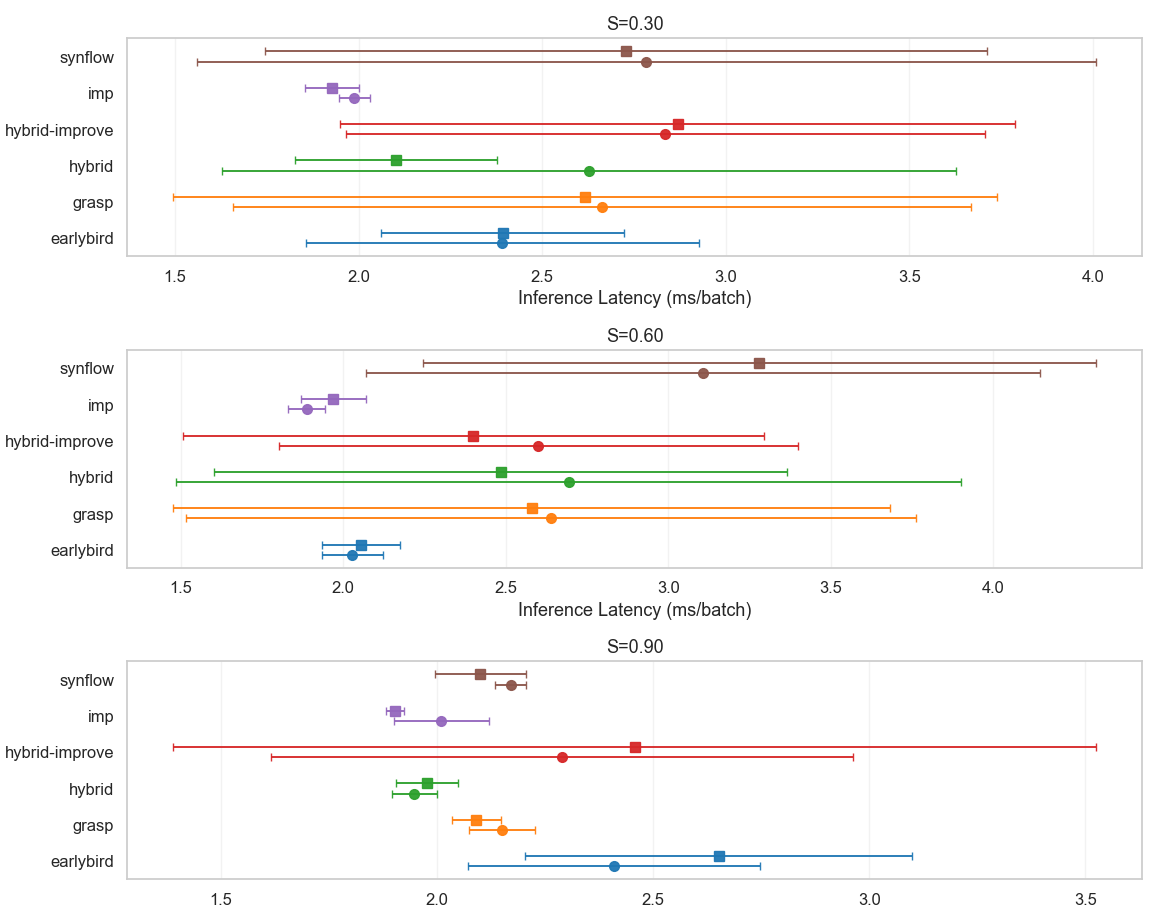
\includegraphics[width=0.7\textwidth]{image/resnet20-cifar100_latency.png}
        \caption{Độ trễ suy diễn theo mức độ thưa trên CIFAR-100/ResNet-20}
        \label{fig:r20c100_latency}
    \end{figure}
}

\frame{
    \frametitle{Thực nghiệm}
    \framesubtitle{Độ trễ suy diễn và chi phí huấn luyện}
    \begin{figure}[h]
        \centering
        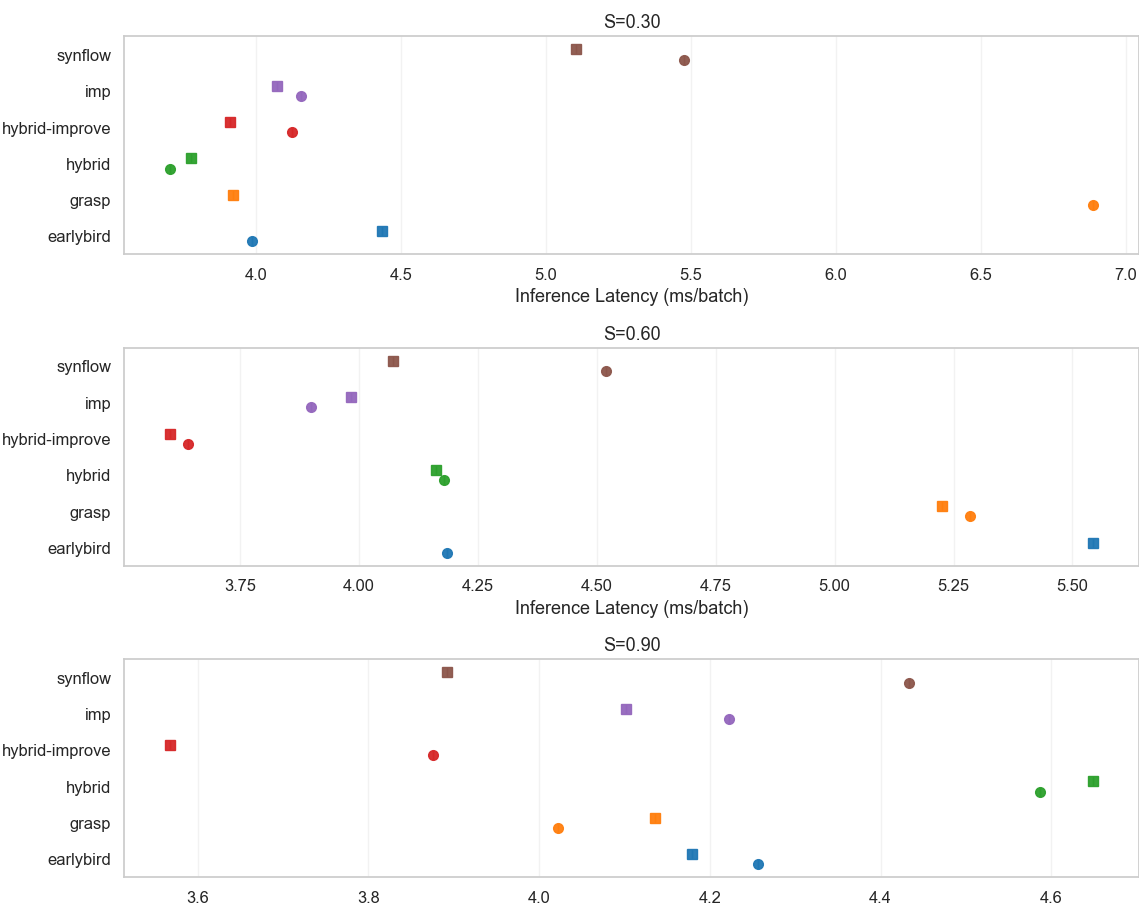
\includegraphics[width=0.68\textwidth]{image/resnet50-cifar10_latency.png}
        \caption{Độ trễ suy diễn theo mức độ thưa trên CIFAR-10/ResNet-50}
        \label{fig:r50c10_latency}
    \end{figure}
}


\frame{
    \frametitle{Thực nghiệm}
    \framesubtitle{Độ trễ suy diễn và chi phí huấn luyện}
    \textbf{Độ trễ suy diễn (ms/batch):}
    \begin{itemize}
        \item Ở $S=0.30$ và $S=0.60$: thanh lỗi rải rộng $>2$ ms -- sự khác biệt dense vs. pruned nằm trong \textbf{vùng nhiễu đo lường}
        \item Ở $S=0.90$: thanh lỗi thu hẹp ($\pm 0.1$--$0.3$ ms), nhưng sự khác biệt cũng biến mất $\Rightarrow$ cắt tỉa không có cấu trúc (unstructured) \textbf{không giảm độ trễ thực tế} trên phần cứng thông thường
    \end{itemize}
    \vspace{0.3cm}
    \textbf{Chi phí huấn luyện:}
    \begin{itemize}
        \item \textbf{IMP}: đắt nhất ($10^4$--$10^5$ giây) do nhiều vòng prune-retrain-rewind
        \item \textbf{GraSP / SynFlow}: rẻ nhất (1 lần cắt tỉa + 1 lần huấn luyện)
        \item \textbf{Hybrid / Hybrid-Improve}: mức trung gian, biến động theo khi nào early stopping kích hoạt
    \end{itemize}
}

%%%%%%%% 5. KẾT LUẬN %%%%%%%%

\section{Kết luận}

\frame{
    \frametitle{Kết luận}
    \framesubtitle{Tổng kết đóng góp}
    \textbf{Hai đóng góp chính:}
    \begin{enumerate}
        \item \textbf{Biến thể Hybrid-Improve} với ba cải tiến:
        \begin{itemize}
            \item Xác định $r_k$ động qua Fisher Information Trace
            \item Chưng cất tri thức từ mô hình gốc sau bước cắt tỉa lớn
            \item Lịch warm-up tuyến tính ở đầu mỗi vòng lặp hình học
        \end{itemize}
        \item \textbf{Phân tích thực nghiệm toàn diện} trên ResNet-20/50 và CIFAR-10/100
    \end{enumerate}
    \vspace{0.3cm}
    \textbf{Kết quả nổi bật:}
    \begin{itemize}
        \item Hybrid-Improve: mức sụt giảm thấp nhất ở \textbf{độ thưa vừa phải}
        \item Hybrid-Improve: \textbf{ổn định nhất} qua nhiều lần chạy ở tất cả mức độ thưa
        \item Trên ResNet-50 tại $S=0.90$: GraSP cạnh tranh trên biên Pareto (accuracy vs. chi phí)
        \item Early-Bird: không phù hợp cho $S \geq 0.60$, đặc biệt trên CIFAR-100
    \end{itemize}
}

\thispagestyle{empty}
\begin{frame}[c]
\begin{center}
\LARGE{\textbf{XIN CHÂN THÀNH CẢM ƠN!}}
\end{center}
\end{frame}

\end{document}